\NeedsTeXFormat{LaTeX2e}

% The following saves the original definitions of \geq and \leq (guide only).
\let\realgeq\geq
\let\realleq\leq

\documentclass{fac}

\ifprodtf \else \usepackage{latexsym}\fi

% The following macros automatically define symbols to be used in Table 1 of
% the authors' guide, using characters from the AMS symbol font MSAM.

\newcommand\black{\ensuremath{\blacktriangleright}}
\newcommand\white{\ensuremath{\vartriangleright}}

\newif\ifamsfontsloaded
\ifprodtf
  \newcommand\whbl{\white\kern-.1em--\kern-.1em\black}
  \newcommand\blwh{\black\kern-.1em--\kern-.1em\white}
  \newcommand\blbl{\black\kern-.1em--\kern-.1em\black}
  \newcommand\whwh{\white\kern-.1em--\kern-.1em\white}
  \amsfontsloadedtrue
\else
  \checkfont{msam10}
  \iffontfound
    \IfFileExists{amssymb.sty}
      {\usepackage{amssymb}\amsfontsloadedtrue
       \newcommand\whbl{\white\kern-.125em--\kern-.125em\black}%
       \newcommand\blwh{\black\kern-.125em--\kern-.125em\white}%
       \newcommand\blbl{\black\kern-.125em--\kern-.125em\black}%
       \newcommand\whwh{\white\kern-.125em--\kern-.125em\white}}
      {}
  \fi
\fi

%% Macros for the guide only %%
\newcommand\eg{\textit{e.g.\ }}
\newcommand\ie{\textit{i.e.\ }}
\newcommand\etc{\textit{etc}}
\newcommand\hatp{\skew3\hat{p}}
\newcommand\lra{\ensuremath{\quad\longrightarrow\quad}}
\providecommand\AMSLaTeX{AMS\,\LaTeX}
%% End of macros for the guide %%

\newtheorem{theorem}{Theorem}[section]

\title{TFA: An Efficient and Precise Virtual Method Call Resolution for Java}

\author[Xilong Zhuo and Chenyi Zhang]
    {Xilong Zhuo$^\star$ and Chenyi Zhang$^\star$\\
     $^\star$College of Information Science and Technology, Jinan University, Guangzhou, China\thanks{A preliminary version appears in the proceedings of the $21$st International Conference on Formal Engineering Methods (ICFEM 2019) held in Shenzhen, China, November 5th-9th, 2019.}}

\correspond{Chenyi Zhang.
            e-mail: chenyi\_zhang@jnu.edu.cn}

%\pubyear{2000}
\pagerange{\pageref{firstpage}--\pageref{lastpage}}

\newtheorem{Definition}{Definition}
\newtheorem{Theorem}{Theorem}
\newtheorem{Lemma}{Lemma}
\newtheorem{Property}{Property}
\newtheorem{Corollary}{Corollary}
\newtheorem{Proof}{Proof}
\newtheorem{Example}{Example}

\newcommand{\keyword}[1]{\mathsf{#1}}
\newcommand{\kw}[1]{\keyword{#1}}

\newcommand{\kwnull}[0]{\keyword{null}}
\newcommand{\kwnew}[0]{\keyword{new}}
\newcommand{\kwextends}[0]{\keyword{extends}}
\newcommand{\kwclass}[0]{\keyword{class}}
\newcommand{\kwthis}[0]{\keyword{this}}
\newcommand{\kwif}[0]{\keyword{if}}
\newcommand{\kwthen}[0]{\keyword{then}}
\newcommand{\kwelse}[0]{\keyword{else}}
\newcommand{\kwskip}[0]{\keyword{skip}}

\newcommand\Var{\mathtt{VAR}}
\newcommand\Val{\mathtt{V}}
\newcommand\Obj{\mathtt{OBJ}}

\newcommand{\VPT}{\Omega}
\newcommand{\HPT}{\Phi}
\newcommand{\Class}{\mathcal{C}}
\newcommand{\Field}{\mathcal{F}}
\newcommand{\bigO}{\mathcal{O}}
\newcommand{\word}[1]{\langle #1\rangle}
\newcommand{\Nat}{\mathbb{N}}
\newcommand{\less}{\sqsubseteq}
\newcommand{\tflow}{\dashrightarrow}
\newcommand{\hflow}{\longrightarrow}
\newcommand{\lhflow}[1]{\stackrel{#1}{\hflow}}
\newcommand{\lhflowstar}[1]{\stackrel{#1}{\longrightarrow^*}}

\newcommand\Loc{\mathcal{L}}
\newcommand\Label{\Phi}
\newcommand\set[1]{\{#1\}}
\newcommand\power{\mathcal{P}}
\newcommand\join{\cup}
\newcommand\subtype{\subseteq}

\usepackage{amsfonts}
\usepackage{amsmath}
\usepackage{amssymb}
\usepackage{threeparttable}
\usepackage{graphicx}
\usepackage{color}
\usepackage{verbatimbox}
\usepackage{url}
\usepackage{subfigure}
\usepackage{multirow}

\definecolor{lbcolor}{rgb}{1,1,1}

\usepackage{listings}
\lstset{
  backgroundcolor=\color{lbcolor},
  language=java,
  frame=single,
  numbers=left,
  stepnumber=1,
  firstnumber=1,
  numberfirstline=true,
  tabsize=4,
  captionpos=b,
  keywordstyle=\color[rgb]{0,0,1},
  commentstyle=\color[rgb]{0.133,0.545,0.133},
  stringstyle=\color[rgb]{0.627,0.126,0.941}
}

\begin{document}
\label{firstpage}

\makecorrespond

\maketitle

\begin{abstract}
The problem of statically resolving virtual method calls in object-oriented (OO) programming languages has been a long standing challenge, often due to the overly complicated class hierarchy structures in modern OO programming languages such as Java, C$\#$ and C++. Traditional ways of dealing with this problem include class hierarchy analysis (CHA), variable type analysis (VTA), and retrieval of type information after a sophisticated points-to analysis. In this paper, we tackle this problem by proposing a new approach called type flow analysis (TFA) which propagates type information as well as field access information through the syntactic structure of a program. Our methodology is purely algebraic and there is no need to explicitly construct a heap abstraction.

We have assessed our methodology from two perspectives. Regarding its theoretical foundation, we have proved that in the context insensitive setting, our method is as precise as the standard Andersen's subset-based points-to analysis regarding the derived types for variables. For an experimental evaluation of TFA, we have implemented the algorithm in the Soot framework and used it to analyze the SPECjvm2008 benchmark suite. During the experiment, we have shown that our method is usually $30-100$ times faster than the standard points-to analysis. We further conduct a range of detailed analysis based on the baseline data obtained by running a dynamic profiler, which is also implemented by us, on the SPECjvm2008. The experiment results confirm that TFA can achieve outstanding performance with acceptable accuracy when applied on real world Java programs.


%The problem of resolving virtual method and interface calls in object-oriented languages has been a long standing challenge to the program analysis community. The complexities are due to various reasons, such as increased levels of class inheritance and polymorphism in large programs. In this paper, we propose a new approach called type flow analysis that represent propagation of type information between program variables by a group of relations without the help of a heap abstraction. We prove that regarding the precision on reachability of class information to a variable, our method produces results equivalent to that one can derive from a points-to analysis.
%Moreover, we implement a static type analysis tool for our approach. To evaluate our method, we use instrumentation tenichque to implement a dynamic profiling type recorder. The experimental results show that our approach is more practical in both efficiency and accuracy.
\end{abstract}

\begin{keywords}
Type Analysis; Static Analysis; Virtual Method Resolution; Call Graph Construction
\end{keywords}

\section{Introduction}\label{sec:introduction}
For object-oriented programming languages, virtual methods (or functions) are those declared in a base class but are meant to be overridden independently in child classes. Statically determine a set of methods that may be invoked at a call site is of vital importance to program optimization. From results of a precise static method call resolution, a subsequent optimization process may be applied to reduce the cost of virtual function calls, or to perform method inlining if target method forms a singleton set. From these results one may also remove methods that are never called by any call sites (\ie dead code elimination), or produce a call graph which can be useful in other optimization~processes.

Efficient solutions, such as Class Hierarchy Analysis (CHA)~\cite{Dean1995,Fernandez1995} and Rapid Type Analysis (RTA)~\cite{Bacon1996}, conservatively assign each variable a set of class definitions, with relatively low precision. Variable Type Analysis (VTA)~\cite{Sundaresan2000} collects types from the object instantiation sites and then propagates type information within the program. However, VTA does not differentiate variables of the same class, which potentially causes imprecision. Alternatively, with the help of a heap abstraction, one may take advantage of points-to analysis~\cite{andersen94} to compute a set of objects that a variable may refer to, and resolve the receiver classes by retrieving the types of the objects, before determining associated methods at call sites.

In general, the algorithms used by CHA, RTA and VTA are conservative, which aim to provide an efficient way to resolve calling edges, and which usually take linear-time in the size of a program, by focusing on the types that are collected at the receiver of a call site. For instance, let $x$ be a variable of declared class $A$, then at a call site $x.m()$, CHA will draw a call edge from this call site to method $m()$ of class $A$ and every definition $m()$ of a class that extends $A$. In case class $A$ does not define $m()$, a call edge to an ancestor class that defines $m()$ will also be included. For a variable $x$ of declared interface $I$, CHA will draw a call edge from this call site to every method of name $m()$ defined in class $X$ that implements $I$.
We write $CHA(x,m)$ for the set of methods that are connected from call site $x.m()$ as resolved by  Class Hierarchy Analysis (CHA).
Rapid Type Analysis (RTA) is an improvement from CHA which resolves call site $x.m()$ to $CHA(x,m)\cap inst(P)$, where $inst(P)$ stands for the set of methods of classes that are (syntactically) instantiated in the program.

\begin{figure}
\begin{minipage}[t]{0.5\linewidth}
\centering
\begin{verbbox}
class A{
    A f;
    A m(){
        return this.f;
    }
}

class B extends A{}

class C extends A{}
\end{verbbox}
\theverbbox
\end{minipage}
\begin{minipage}[t]{0.5\linewidth}
%\center
\centering
\begin{verbbox}
1:  A x = new A();  //O_1
2:  B b = new B();  //O_2
3:  A y = new A();  //O_3
4:  C c = new C();  //O_4
5:  x.f = b;
6:  y.f = c;
7:  z = x.m();
\end{verbbox}
\theverbbox
\end{minipage}
\caption{An example that compares precision on type flow in a program.}\label{figure:example}
\end{figure}

Variable Type Analysis (VTA) is a further improvement. VTA defines a node for each variable, method, method parameter and field. Class names are treated as values and propagation of such values between variables work in the way of value flow.
As shown in Figure~\ref{figure:vta} (example code in Figure~\ref{figure:example}), the statements on line $1-4$ of Figure~\ref{figure:example} initialize type information for variables $x$, $y$, $b$ and $c$, and statements on line $5-7$ establish value flow relations. Since both $x$ and $y$ are assigned type $A$, $x.f$ and $y.f$ are both represented by node $A.f$, thus the set of types reaching $A.f$ is now $\set{B,C}$. (Note this is a more precise result than CHA and RTA which assign $A.f$ with the set $\set{A,B,C}$.)
Since $A.m.this$ refers to $x$, $this.f$ inside method $A.m()$ now refers to $A.f$. Therefore, through $A.m.return$, $z$ receives  $\set{B,C}$ as its final set of reaching types.

\begin{figure}%%[ht]
\begin{tabular}{cc}

\begin{minipage}[h]{0.5\linewidth}
\centering
\begin{tabular}{|c|c|}
  \hline
  \textbf{Statement} & \textbf{VTA fact} \\
   \hline
  \hline
  % after \\: \hline or \cline{col1-col2} \cline{col3-col4} ...
  $A\ x = \kwnew\ A()$ & $x\leftarrow A$ \\ \hline
  $B\ b = \kwnew\ B()$ & $b\leftarrow B$ \\ \hline
  $A\ y = \kwnew\ A()$ & $y\leftarrow A$ \\ \hline
  $C\ c = \kwnew\ C()$ & $c\leftarrow C$ \\ \hline
  $x.f = b$ & $A.f\leftarrow b$ \\ \hline
  $y.f = c$ & $A.f\leftarrow c$ \\ \hline
   & $A.m.this\leftarrow x$ \\
  $z = x.m()$  & $A.m.return\leftarrow A.f$ \\
   & $z\leftarrow A.m.return$\\
  \hline
\end{tabular}
\caption{VTA facts on the example}\label{figure:vta}
\end{minipage}
&
\begin{minipage}[h]{0.5\linewidth}
\centering
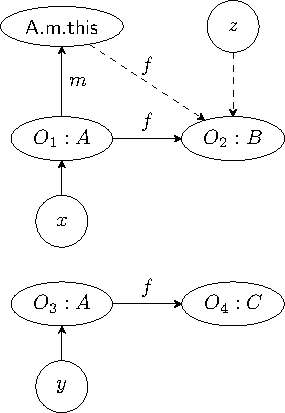
\includegraphics[width=3.5cm]{points-to.pdf}
\caption{Points-to results on the example}\label{figure:points-to}
\end{minipage}
\end{tabular}
\end{figure}

The result of a context-insensitive subset based points-to analysis~\cite{andersen94} creates a heap abstraction of four objects (shown on line $1-4$ of Figure~\ref{figure:example} as well as the ellipses in Figure~\ref{figure:points-to}). These abstract objects are then inter-connected via field store access defined on line $5-6$. The derived field access from $A.m.this$ to $O_2$ is shown in dashed arrow. By return of the method call $z=x.m()$, variable $z$ receives $O_2$ of type $B$ from $A.m.this.f$, which gives a more precise set of reaching types for variable $z$.

From this example, one may conclude that the imprecision of VTA in comparison with points-to analysis is due to the over abstraction of object types, such that $O_1$ and $O_3$, both of type $A$, are treated under the same type. Nevertheless, points-to analysis requires to construct a heap abstraction, which brings in undersirable extra information when we are only interested in the set of reaching types of a variable.

\begin{figure}
\centering
%\vspace{5cm}
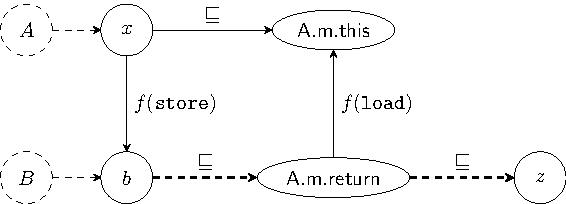
\includegraphics[width=8cm]{tfa.pdf}
\caption{Type Flow Analysis for variable $z$ in the example}\label{fig:tfa}
\end{figure}

In this paper we introduce a relational static semantics called Type Flow Analysis (TFA) on program variables and field accesses. Different from VTA, in addition to the binary value flow relation ``$\less$'' on the variable domain $\Var$, where $x\less y$ denotes all types that flow to $x$ also flow to $y$, we also build a ternary field store relation $\rightarrow\ \subseteq\Var\times\Field\times\Var$ to trace the \emph{load} and \emph{store} relationship between variables via field accesses. This provides us additional ways to extend the relations $\less$ as well as $\rightarrow$. %%For example given $x\lhflow{f}y$ and $x\less z$, we can derive $z\lhflow{f}y$.
%%
Taking the example from Figure~\ref{figure:example}, we are able to collect the store relation $x\lhflow{f}b$ from line $5$. Since $x\less \textsf{A.m.this}$, together with the implicit assignment which loads $f$ of $\textsf{A.m.return}$, we further derives $b\less\textsf{A.m.return}$ and $b\less z$ (dashed thick arrows in Figure~\ref{fig:tfa}). Therefore, we assign type $B$ to variable $z$. The complete reasoning pattern is depicted in Figure~\ref{fig:tfa}. Nevertheless, one cannot derive $c\less z$ in the same way.

%%% contributions with %%% discussion on context-sensitivity
We have proved that in the context-insensitive inter-procedural setting, TFA is as precise as the subset based points-to analysis (which we refer to as PTA in the rest of the paper) regarding type related information. Since points-to analysis can be enhanced with various types of context-sensitivity on variables and objects (\eg, call-site-sensitivity~\cite{Shivers91,Kastrinis2013}, object-sensitivity~\cite{Milanova2005,Smaragdakis11,Tan16} and type-sensitivity~\cite{Smaragdakis11}), extending type flow analysis with context-sensitivity will only require to consider contexts on variables, which is left for future work.

We have implemented a static type analysis tool for context-insensitive type flow analysis, which is written in Java and aims to analyze Java programs. We run our algorithm on the jimple IR, a typed, 3-address, statement based intermediate representation provided by Soot framework~\cite{soot}. The implementation has been tested on a collection of benchmark programs from SPECjvm2008~\cite{specjvm}. We conducted several experiments to compare TFA regarding efficiency and accuracy with CHA and PTA implemented by the Soot team. In order to establish a reliable comparison regarding \emph{precision} and \emph{recall} of different approaches, we apply the instrumentation technique to implement a dynamic profiling tool for jimple, which extracts types of callee method at runtime. We then conduct a sophisticated study on the different static approaches regarding results generated by the dynamic profiler. The experimental result has shown that TFA is in general more efficient than PTA. In terms of accuracy, TFA is more precise than CHA. Note that due to the comprehensive optimizations for VTA and PTA that are implemented by the Soot team, a decent comparison to the VTA and PTA implementation available in Soot is not straightforward. We have tried to create a relatively suitable environment by disabling some of the optimizations in Soot, and eventually reach the conclusion that the precision of TFA is comparable to VTA and PTA regarding the SPECjvm2008 benchmark suite. In addition, we confirm that most existing approaches, including PTA and TFA, do not guarantee soundness on all benchmarks, as already discussed in the literature~\cite{LivshitsSSLACGKMV15}. We then look into all the unmatch record to find out the source of imprecision and unsoundness, with short discussions regarding the related Java language features such as JDK library calls, Java reflection API, Java Native Interface and the callback mechanism. %%%We will discuss it in the experiment section of this paper. %(Need more citations here, and brief the experimental results.)
Our implementation is publicly available at \url{https://github.com/SeanCoek/tfa}.

Over all the contributions of the paper are listed as follows.
\begin{enumerate}
  \item We have proposed a new relational static semantics called Type Flow Analysis (TFA), which computes a collection of reachable types for variables. Our methodology is enforced by type propagation via value flow between program variables as well field accesses, following predefined relational rules (C.f.~Definition~\ref{def:base} and Definition~\ref{def:extension}). We have proved equivalence between TFA and the subset based points-to analysis regarding collected types for variables (Theorem~\ref{thm:tfa}), presented in Section~\ref{sec:type-flow-analysis}.
  \item We have implemented the TFA algorithm in the Soot framework, and conducted a comprehensive study regarding performance and accuracy. The detailed description regarding the implementation and comparison with existing approaches (CHA, VTA and PTA) are presented in Section~\ref{sec:implementation} and Section~\ref{sec:evaluation}.
  \item As a byproduct, we have implemented a dynamic profiler, by instrumenting code that collects at each call site a set of types of the receiver variable as well as callee methods. The collected type information serves as a baseline for measuring and comparing the precisions between TFA and the aforementioned virtual method call resolution algorithms.
\end{enumerate}

\section{Type Flow Analysis}\label{sec:type-flow-analysis}

We define a core calculus consisting of most of the key object-oriented language features, shown in Figure~\ref{fig:syntax}, which is designed in the same spirit as Featherweight Java~\cite{Igarashi2001}.
A program is defined as a code base $\overline{C}$ (i.e., a collection of class definitions) with statement $s$ to be evaluated.
To run a program, one may assume that $main$ is the default (static) entry method with local variable declarations $\overline{D}$,
similar to e.g., Java and C++, which may differ in specific language designs.
%% to consider dynamic semantics later: Let $S$ and $H$ be the runtime stack and heap, where $S:\Var\rightarrow \Val$maps local variables to values and $H:\Val\rightarrow \Obj\cup\set{\kwnull}$ maps values to objects.
We define a few auxiliary functions. Let function $fields$ maps class names to their fields, $methods$ maps class names to their defined or inherited methods, and $type$ provides types (or class names) for objects. Given class $c$, if $f\in fields(c)$, then $ftype(c,f)$ is the defined class type of field $f$ in $c$. Similarly, give an object $o$, if $f\in fields(type(o))$, then $o.f$ may refer to an object of type $ftype(type(o),f)$ or %%an object of
any of its subclass at runtime. Write $\Class$ for the set of classes, $\Obj$ for the set of objects, $\Field$ for the set of fields and $\Var$ for the set of variables that appear in a program.
\footnote{Sometimes we mix-use the terms \emph{type} and \emph{class} in this paper when it is clear from the context.}

\begin{figure}\centering
	\begin{tabular}[c]{lll}
		$C$&$::=$&$\kwclass\ c\ [\kwextends\ c'] \ \{\overline{F};\ \overline{M}\}$\\
        $F$&$::=$&$c \ f$\\
        $D$&$::=$&$c \ z$\\
		$M$&$::=$&$m(x) \ \{\overline{D}; s; \kw{return}\ x'\}$\\
		$s$&$::=$&$x{=}\kwnew \ c\mid  x {=} e \mid x.f{=}y \mid s;s$\\

		$e$&$::=$&$ \kwnull\mid x \mid x.f \mid x.m(y) $\\
        $prog$&$::=$&$\overline{C};\overline{D}; main$\\
	\end{tabular}
	\caption{Abstract syntax for the core language. \label{fig:syntax}}
\end{figure}

In this simple language we do not model common types (\eg, int and float) that are irrelevant to our analysis. We focus on the reference types which form a class hierarchical structure. We assume a context insensitive setting, such that every variable can be uniquely determined by its name together with its enclosing class and method.
For example, if a local variable $x$ is defined in method $m$ of class $c$, then $c.m.x$ is the unique representation of that variable. Therefore, it is safe to drop the enclosing class and method name if it is clear from the context.
In general, we have the following types of variables in our analysis: (1) local variables, (2) method parameters, (3) \texttt{this} reference of each method, all of which are syntactically bounded by their enclosing classes and methods.

We define three relation for catching type flow information in programs, a partial order on variables $\less\ \subseteq\Var\times\Var$, a type flow relation
$\tflow\subseteq\Class\times\Var$, as well as a field access relation $\hflow\subseteq\Var\times\Field\times\Var$,
which are initially given as follows.

%\paragraph{Definition 1.}
\begin{Definition}\label{def:base} (Base Relations)
These three base relations represent program facts which are generated directly %based on different
from statements syntactically appearing in programs.
\begin{enumerate}
  \item $c\tflow x$ if there is a statement $x = \kwnew\ c$;
  \item $y\less x$ if there is a statement $x = y $;
  \item $x\lhflow{f}y$ if there is a statement $x.f = y$.
\end{enumerate}
\end{Definition}

Intuitively, $c\tflow x$ means variable $x$ may have type $c$ (\ie $c$ flows to $x$), $y\less x$ means all types that flow to $y$ also flow to $x$, and $x\lhflow{f}y$ means that one may access variable $y$ from field $f$ together with variable $x$.\footnote{Note that VTA treats statement $x.f = y$ in a different way as follows. For each class $c$ that flows to $x$ which defines field $f$, VTA assigns all types that flow to $y$ also to $c.f$.}

\begin{Example}\label{ex:def1}
We give a snippet code shown in Listing~\ref{lst:relation} to illustrate the generation of relations. For statement ``$A\ a1=new \ A()$'' and ``$B\ b1=new\ B()$'', we generates two type flow relations ``$A \tflow a1$'' and ``$B \tflow b1$'', respectively. We also generate ``$a1 \less a2$'' and ``$a2 \less a3$'' from statements ``$a2=a1$'' and ``$a3=a2$''. For the field store statement on line $6$, we generate a field access relation ``$a1 \lhflow{f} b1$''. The resulting base relations are shown in Figure.~\ref{fig:basic-relation}, where dashed circles refer to types and solid nodes in gray colour represent variables. The type relation, partial order relation and field access relation are shown in dashed arrows, solid arrows labelled ``$\less$'' and solid arrows labelled with field names.
\end{Example}
\begin{minipage}{\linewidth}
\vspace{10pt}
\begin{lstlisting}[caption={An example showing the generation of base relations},label={lst:relation}]
public void m() {
	A a1 = new A();
	a2 = a1;
	a3 = a2;
	B b1 = new B();
	a1.f = b1;
	b2 = a1.f;
	a4 = b2.m2(a3);
}

class B {
	public A m2(p1) {... return r;}
}
\end{lstlisting}
\end{minipage}

\begin{figure}
\centering
\subfigure[Basic relation for Listing~\ref{lst:relation}] {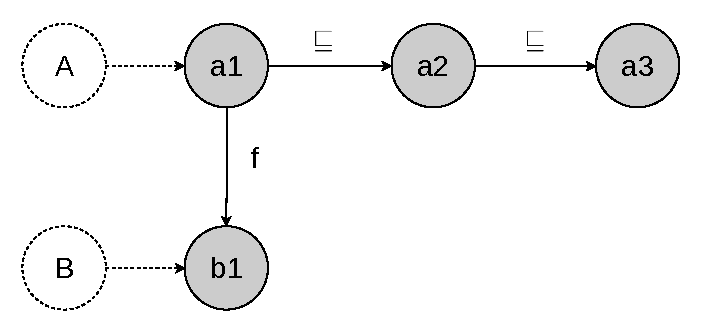
\includegraphics[scale=0.5]{basic-relation.pdf} \label{fig:basic-relation}}
\hspace{2cm}
\subfigure[Extended relation by Definition~\ref{def:extension}(1)] {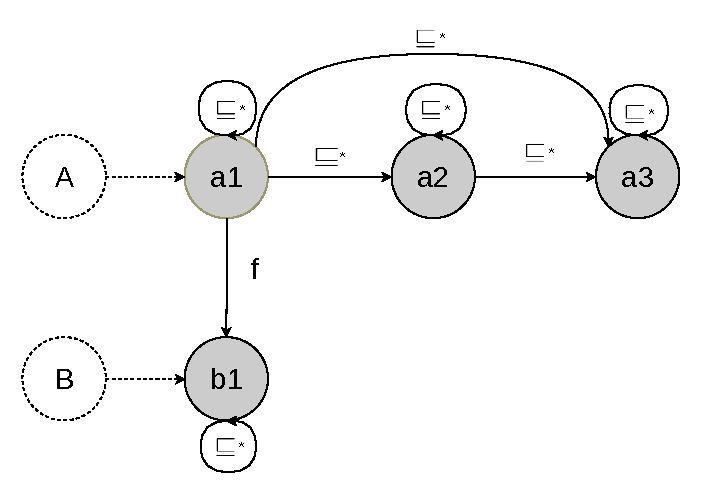
\includegraphics[scale=0.5]{extend-partial.pdf} \label{fig:extend-partial}}
\hspace{2cm}
\subfigure[Extended relation by Definition~\ref{def:extension}(2)] {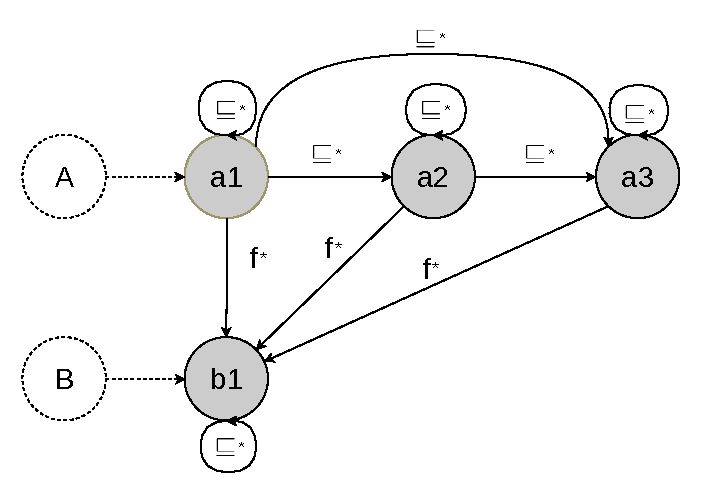
\includegraphics[scale=0.5]{extend-field-access.pdf} \label{fig:extend-field-access}}
\hspace{2cm}
\subfigure[Extended relation by Definition~\ref{def:extension}(3)] {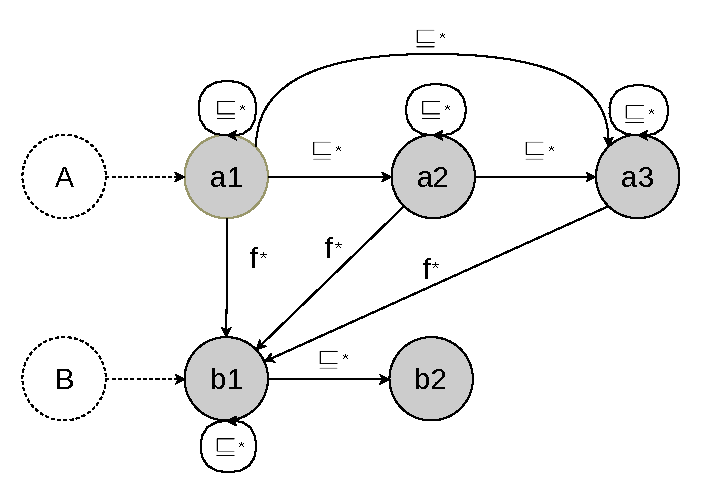
\includegraphics[scale=0.5]{extend-field-load.pdf} \label{fig:extend-field-load}}
\hspace{2cm}
\subfigure[Extended relation by Definition~\ref{def:extension}(4)] {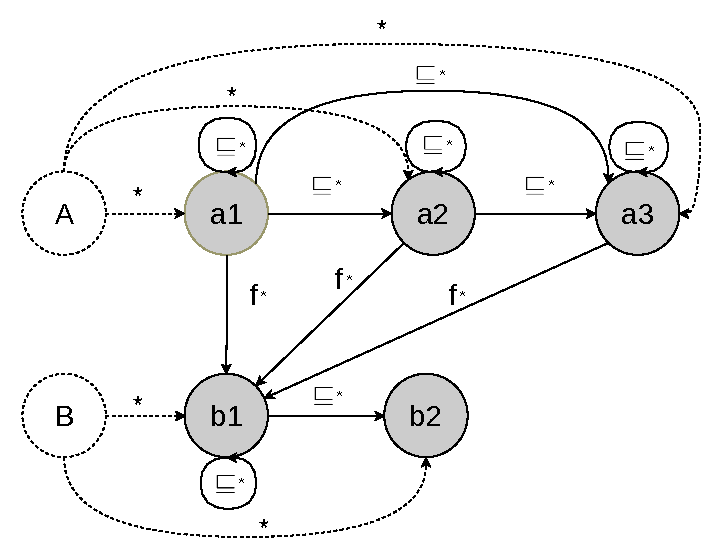
\includegraphics[scale=0.5]{extend-type-flow.pdf} \label{fig:extend-type-flow}}
\hspace{2cm}
\subfigure[Extended relation by Definition~\ref{def:extension}(5)] {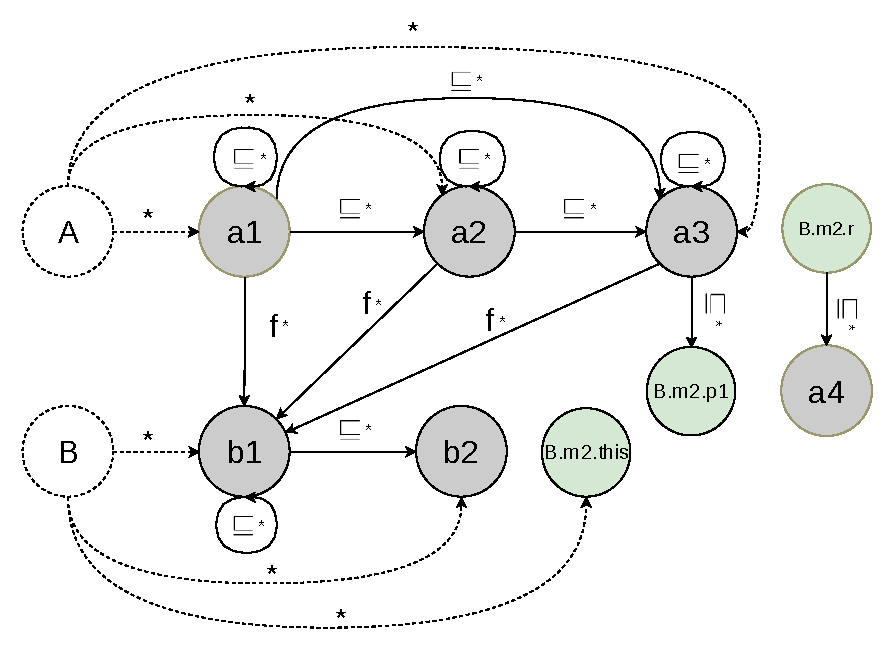
\includegraphics[scale=0.5]{extend-invocation.pdf} \label{fig:extend-invocation}}
\caption{One round of relation generation for method $m()$ in Listing~\ref{lst:relation}}
\label{fig:relations}
\end{figure}

%We use five rules to extend the basic relations for  calculating a program fixpoint, which are given in the following definition 2. These rules intuitively represent propagation of type information. We put a `$^*$' label behind relation symbol to destinguish from basic relations.

In the following we define extended relations to capture propagation of type information inter-procedurally in programs. As a convention, $R^*$ (Kleene star) is used to represent the reflexive and transitive closure of relation $R$. Then we explain the associated operations in Example~\ref{ex:def2}, illustrated~in~Figure~\ref{fig:relations}.

\begin{Definition}\label{def:extension} (Extended Relations)
\begin{enumerate}
\item $y\less^* x$ if $x=y$ or $y\less x$ or $\exists z\in\Var:y\less^* z\wedge z\less^* x$;

  %This rule is based on the properties of reflexive and transtive since $\less$ is a partial order relation. Besides, $y\less x$ implies $y\less^* x$. Under this rule, we extend the basic relations in~\ref{fig:basic-relation} and show the result in~\ref{fig:extend-partial}.

\item $y\lhflow{f\ *}z$ if $\exists x\in\Var: x\lhflow{f}z\wedge (\exists z'\in\Var: z'\less^* y \wedge z'\less^*x)$;

%  This rule is designed to extending field access relation. Based on the relations we generated in~\ref{fig:extend-partial}, we can generated three $\lhflow{f\ *}$ relations, ``$a1 \lhflow{f\ *} b1$'', ``$a2 \lhflow{f\ *} b1$'' and ``$a3 \lhflow{f\ *} b1$'', as displayed in~\ref{fig:extend-field-access}.

\item For all statements $x = y.f $, if $y\lhflow{f\ *}z$, then $z\less^* x$.

%  For field load statements, only we have generated a relavant field access relation, can we extend $\less^*$ relation for target variables. \eg, From the result of~\ref{fig:extend-field-access}, we have a field access relation ``$a1\lhflow{f\ *} b1$''. So we can generate a relation ``$b1\less^* b2$'' for the field load statement ``$b2=a1.f$'' on line 7 of Listing~\ref{lst:relation}. We put the result on Fig.~\ref{fig:extend-field-load}.

\item $c\tflow^* y$ if $c\tflow y$, or $\exists x\in\Var:c\tflow^* x\wedge x\less^* y$;

%  Intuitively, this rule describe how the type information being propagated over the $\less^*$ relation. We use this rule to extend the relations from~\ref{fig:extend-field-load}. The generated relations are represented in dash arrow with a label of `$^*$', as displayed in~\ref{fig:extend-type-flow}.

\item The type information is used to resolve each method call $x = y.m(z)$.
  \begin{equation*}
  \left.\begin{array}{l}\forall\ c\tflow^* y:\\ \forall\ m(z')\{\dots \kw{return}\ x'\}\in methods(c):\end{array}\right.\left\{\begin{array}{l}
        z\less^* c.m.z'\\
        c\tflow^* c.m.this\\
        c.m.x'\less^* x \\
        \end{array}\right.
  \end{equation*}
\end{enumerate}
\end{Definition}

Regarding the extended relations given in Definition~\ref{def:extension}, we provide the following intuitions. Definition~\ref{def:extension}($1$)  computes the reflexive and transtive closure of the relation $\less$.
In Definition~\ref{def:extension}($2$), with the existence of $z'$, variables $x$ and $y$ are in the \emph{may-alias} relation, therefore, all that is accessible by $x$ via field $f$ is also accessible by $y$ via $f$. This rule is designed to extend the field access relation.
Definition~\ref{def:extension}($3$) loads $z$ to $x$ (via $f$) from $y$, provided that $z$ is accessible by $y$ via $f$.
Definition~\ref{def:extension}($4$) extends the type flow relation by taking advantage of the extended partial order $\less^*$ on variables.
Definition~\ref{def:extension}($5$) deals with inter-procedural type flow, which defines three extensions for parameter variables, \texttt{this} references and \texttt{return} variables, respectively.

%These three kinds of generated relation reprensent the type flow on parameter variables, ``$this$'' reference variable and return variables, respectively.
%The reaching type of variable $b2$ is $\{B\}$, \ie, we have ``$B \tflow^* b2$'', which we can extract from the result of ~\ref{fig:extend-type-flow}. That means statement ``$a4=b2.m2(a3)$'' will trigger the invocation of method $m2()$ in class $B$. In this case, we generated three relations, ``$a3 \less^* B.m2.p1$'', ``$B \tflow^* B.m2.this$'' and ``$B.m2.r \less^* a4$''. The result is shown is ~\ref{fig:extend-invocation}, where variables in method $B.m2()$ is represented as circle in green background.

\begin{Example}\label{ex:def2} %% need to expand by describing functionalities of the rules in Def 2.
We describe the process of generating extended relations for the base model that is discussed in Example~\ref{ex:def1}, as depicted in Figure~\ref{fig:relations}. Although the actual computation may take a number of iterations to reach a fixpoint, to make the process more understandable, we try to sketch in separate how each rule given in Figure~\ref{fig:relations} works. Initially, the base relation for Listing~\ref{lst:relation} is given in Figure~\ref{fig:relations}(a). Definition~\ref{def:extension}($1$) extends the base relation $\less$ into $\less^*$, as shown in Figure~\ref{fig:relations}(b). Definition~\ref{def:extension}($2$) extends the field access relation, resulting in Figure~\ref{fig:relations}(c). By applying Definition~\ref{def:extension}($3$), we further extends $\less^*$ through the existing field access relation, reaching the graph in Figure~\ref{fig:relations}(d). Then Definition~\ref{def:extension}($4$) propagates the type flow relation $\tflow^*$ by considering the existing partial order relation and field access relation on variables, as shown in Figure~\ref{fig:relations}(e). In Figure~\ref{fig:relations}(f) we further enrich the relations for inter-procedural type flow, where the statement ``$a4=b2.m2(a3)$'' triggers the invocation of method $m2()$ in class $B$, from which we establish ``$a3 \less^* B.m2.p1$'', ``$B \tflow^* B.m2.this$'' and ``$B.m2.r \less^* a4$'', where $B.m2.p1$ and $B.m2.r$ are respectively the virtual parameter of method $m2()$ and the return variable of method $m2()$. In fact, Figure~\ref{fig:relations}(f) is very close to the smallest type flow model satisfying all constraints given in Definition~\ref{def:extension} regarding the program in Listing~\ref{lst:relation}.
%
%We show the detailed process of relation generation in one round, as displayed in~\ref{fig:relations}. In general we need more round to calculte a program fixpoint. The final relations are the least relations that satisfy constraints of Definition 2. Although the three relations are inter-dependent, one may find that without method call (i.e., Definition~\ref{def:extension}.5), a smallest model satisfying the two relations $\rightarrow^*$ (field access) and $\less^*$ (variable partial order) can be uniquely determined without considering the type flow relation $\tflow^*$.
\end{Example}


In order to compare the precision of TFA with points-to analysis, we present a brief list of the classical subset-based points-to rules for our language in Figure~\ref{fig:constraints}, in which $\VPT$ (the var-points-to relation) maps a reference to a set of objects it may point to, and $\HPT$ (the heap-points-to relation) maps an object and a field to a set of objects. The points-to rules are mostly straightforward, except that %where
$param(type(o),m))$, $this(type(o),m))$ and $return(type(o),m)$ refer to the formal parameter, \textsf{this} reference and \textsf{return} variable of method $m$ of the class for which object $o$ is declared, respectively.

\begin{figure}%[!htbp]
	\centering %
    \begin{tabular}{|l|c|}
        \hline
    \textbf{statement} \hspace{0.5cm} & \textbf{Points-to constraints} \\
    \hline
    $x = \kwnew\ c$ & $o_i\in\VPT(x)$\\
    \hline
    $x = y $ & $\VPT(y)\subseteq\VPT(x)$\\
    \hline
    $x = y.f $ & $\forall o\in\VPT(y):\HPT(o,f)\subseteq\VPT(x)$\\
    \hline
    $x.f = y $ & $\forall o\in\VPT(x):\VPT(y)\subseteq\HPT(o,f)$\\
    \hline
    $x=y.m(z)$ &
        \(\forall o\in\VPT(y):\left\{\begin{array}{l}
        \VPT(z)\subseteq\VPT(param(type(o),m))\\
        o\in\VPT(this(type(o),m))\\%=\set{o}\\
        \forall x'\in return(type(o),m):\\ \hspace{35pt} \VPT(x')\subseteq\VPT(x) \end{array}\right.\)
        \\
    \hline
	\end{tabular}
\caption{Constraints for an context-insensitive points-to analysis. \label{fig:constraints}}
\end{figure}

To this end we present the first result of the paper, which says type flow analysis has the same precision regarding type based check, such as call site resolution and cast failure check, when comparing with the points-to analysis.

\begin{Theorem}~\label{thm:tfa}
  In the context-insensitive setting, for all variables $x$ and classes $c$, $c\tflow^*x$ in TFA iff there exists an object abstraction $o$ of $c$ such that $o\in\VPT(x)$ in points-to analysis.
\end{Theorem}

\begin{proof} (sketch)
First we assume that for each class $c$, every object creation site $x = \kwnew\ c_i$ at line $i$ defines a mini-type $c_i$, and if the theorem is satisfied in this setting, a subsequent merging of mini-types into class $c$ will preserve the result.

Moreover, we only need to prove the result in the intraprocedural setting (\ie Lemma~\ref{lem:tfa-intra}). Because if in the intraprocedural setting the two systems have the same smallest model for all methods, then at each call site $x=y.m(a)$ both analyses will assign $y$ the same set of classes and thus resolve the call site to the same set of method definitions, and as a consequence, each method body will be given the same set of extra conditions, thus all methods will have the same initial condition for the next round iteration. Therefore, both inter-procedural systems will stabilize at the same model.
\end{proof}

The following lemma focuses on the key part of the proof for Theorem~\ref{thm:tfa}, which shows that TFA and points-to analysis are equivalent regarding reachable types to variables intraprocedurally.

\begin{Lemma}\label{lem:tfa-intra}
In a context-insensitive intraprocedural analysis where each class $c$ only syntactically appears once in the form of $\kwnew\ c$, for all variables $x$ and classes $c$, $c\tflow^*x$ iff there exists an object abstraction $o$ of type $c$ such that $o\in\VPT(x)$.
\end{Lemma}
\begin{proof}
Since those constrains of the points-to analysis establish the smallest model $(\VPT, \HPT)$ with $\VPT:\Var\rightarrow\Obj$ and $\HPT:\Obj\times\Field\rightarrow\power(\Obj)$, and the three relations of type flow analysis also define the smallest model that satisfies Definition~\ref{def:base} and Definition~\ref{def:extension}, we prove that every model established by points-to analysis constraints is also a model of TFA, and vice versa. Then the least model of both systems must be the same, as otherwise it would lead to contradiction.

\medskip

($\star$) For the `only if' part ($\Rightarrow$), we define a function $Reaches(x)=\set{c\mid c\tflow^* x}$ which maps a variable to its reaching types in TFA, and assume a bijection $\xi:\Class\rightarrow\Obj$ that maps each class $c$ to the unique (abstract) object $o$ that is defined (and $type(o)=c$). Then we construct a function $Access:\Class\times\Field\rightarrow\power(\Class)$ and show that $(\xi(Reaches),\xi(Access))$ satisfies the points-to constraints. Define $Access(c,f)=\set{c'\mid x\lhflow{f\ *}y\wedge c\in Reaches(x)\wedge c'\in Reaches(y)}$. We prove the following cases according to the top four points-to constraints in Figure~\ref{fig:constraints}.
\begin{itemize}
\item For each statement $x = \kwnew\ c$, we have $\xi(c)\in\xi(Reaches(x))$, as $c\in Reaches(x)$ by Definition~\ref{def:base}(1);
\item For each statement $x = y$, we have $Reaches(y)\subseteq Reaches(x)$ and $\xi(Reaches(y))\subseteq\xi(Reaches(x))$, as $y\less^*x$ by Definition~\ref{def:base}(2);
\item For each statement $x.f = y$, we have $x\lhflow{f}y$ by Definition~\ref{def:base}(3), therefore $x\lhflow{f}^*y$. We need to show that for all $c\in Reaches(x)$, $\xi(Reaches(y))\subseteq \xi(Access(c,f))$.
      Let $c\in Reaches(x)$, and $c'\in Reaches(y)$, by definition we have $c'\in Access(c,f)$. Therefore $Reaches(y)\subseteq Access(c,f)$. Then consequently,
      $\xi(Reaches(y))\subseteq \xi(Access(c,f))$.

\item For each statement $x = y.f$, for all $c\in Reaches(y)$, we need to show $\xi(Access(c,f))\subseteq\xi(Reaches(x))$, or equivalently, $Access(c,f)\subseteq Reaches(x)$. Let $c'\in Access(c,f)$, then by definition of $Access$, there exist $z$, $z'$ such that $c\in Reaches(z)$, $c'\in Reaches(z')$ and $z\lhflow{f\ *}z'$.
    Since each type is uniquely created in the current setting, \ie there exists a statement $z''= \kwnew\ c$ such that $z''\less^* y$ and $z''\less^* z$. Then by $z\lhflow{f\ *}z'$ and Definition~\ref{def:extension}(2), we have $y\lhflow{f\ *}z'$. Then by $x = y.f$ and Definition~\ref{def:extension}(3), we have $z'\less^*x$. Therefore $c'\in Reaches(x)$.
\end{itemize}

\medskip

($\star$) For the `if' part ($\Leftarrow$), let ($\VPT$, $\HPT$) be a model that satisfies all the top four constraints defined in Figure~\ref{fig:constraints}, and a bijection $\xi:\Class\rightarrow\Obj$ between class names and objects, we show that the following constructed relations ($\tflow^*$, $\less^*$, $\lhflow{*}$) derived from ($\VPT$, $\HPT$) satisfy the (intraprocedural) constraints defined for the base relations (\ie Definition~\ref{def:base} and the extended relations (\ie Definition~\ref{def:extension}) for TFA.
\begin{itemize}
  \item For all types $c$ and variables $x$, $c\tflow^* x$ iff $\xi(c)\in\VPT(x)$;
  \item For all variables $x$ and $y$, $x\less^*y$ iff $\VPT(x)\subseteq\VPT(y)$;
  \item For all variables $x$ and $y$, and for all fields $f$, \begin{itemize}
    \item $x\lhflow{f}y$ iff for all $o\in\Obj$, $o\in\VPT(x)$ implies $\VPT(y)\subseteq\HPT(o,f)$.
    \item $x\lhflow{f\ *}y$ iff there exists $o\in\VPT(x)$, $\VPT(y)\subseteq\HPT(o,f)$.
  \end{itemize}
\end{itemize}
We check the following cases for the three relations $\tflow^*$, $\less^*$ and $\lhflow{*}$ that are defined from the above.
\begin{itemize}
\item[-] \textbf{Def~\ref{def:base}(1).} For each statement $x = \kwnew\ c$, we have $\xi(c)\in\VPT(x)$, so $c\tflow^* x$ by definition.
\item[-] \textbf{Def~\ref{def:base}(2).} For each statement $x = y$, we have $\VPT(y)\subseteq\VPT(x)$, therefore $y\less^*x$ by definition.
\item[-] \textbf{Def~\ref{def:base}(3).} For each statement $x.f = y$, we have for all $o_1\in\VPT(x)$ and $o_2\in\VPT(y)$, $o_2\in\HPT(o_1,f)$, which derives $x\lhflow{f\ *}y$ by definition.
\item[-] \textbf{Def~\ref{def:extension}(1).} It is obvious that $\less^*$ is transitive and reflexive, which is by $\subseteq$ being transitive and reflexive.
\item[-] \textbf{Def~\ref{def:extension}(2).} W.l.o.g., for all $x\in\Var$, $\VPT(x)\neq\emptyset$, since the included type could be from $\kwnew$, or from method parameter passing or return. Given $x\lhflow{f}z$, $z'\less^*y$ and $z'\less^*x$, we need to show $y\lhflow{f\ *}z$.
    Let $\xi(c)\in\VPT(z')$, then $\xi(c)\in\VPT(x)$ and $\xi(c)\in\VPT(y)$. Then $\VPT(z)\subseteq\HPT(\xi(c),f)$ by $\xi(c)\in\VPT(x)$ and $x\lhflow{f}z$. Therefore we have $y\lhflow{f\ *}z$ by the existence of $\xi(c)$.

\item[-] \textbf{Def~\ref{def:extension}(3).} For each statement $x = y.f$, given $y\lhflow{f\ *}z$, we need to show $z\less^* x$. Equivalently, by definition there exists $o\in\VPT(y)$ such that $\VPT(z)\subseteq\HPT(o_1,f)$. Given the statement $x = y.f$, for all $o'\in \VPT(y)$ $\HPT(o',f)\subseteq\VPT(x)$, therefore by existence of $o$, we have $\VPT(z)\subseteq\VPT(x)$, the definition of $z\less^* x$.
\item[-] \textbf{Def~\ref{def:extension}(4).} The first case that $c\tflow y$ implies $c\tflow^* y$ is trivial. Let $c\tflow^* x$ and $x\less^*y$, we need to show that $c\tflow^*y$. Since $\xi(c)\in\VPT(x)$ and $\VPT(x)\subseteq\VPT(x)$, we have $\xi(c)\in\VPT(y)$, which is equivalent to $c\tflow^*y$, as required.
\end{itemize}
\end{proof}


\section{Implementation}\label{sec:implementation}
The analysis algorithm is written in Java, and is implemented in the Soot framework, the most popular static analysis framework for Java. We use jimple as intermediate representation (IR).
We do not take common types (\eg, \texttt{int} and \texttt{float}) under our consideration, since these are irrelevant to our analysis.
Our work consists of two parts. The first part implements the static type flow analysis algorithm introduced in previous sections, based on the information extracted from jimple IR and computes a set of types for each reference variable in the program. The second part instantiates a dynamic profiler that collects type-related information, which is then used to analyze precision and recall of the TFA static analysis algorithm, as well as making comparison to other type analysis algorithms including CHA, VTA and PTA. A more detailed description is given as follows, in Section~\ref{subsec:static-analysis-tool} and Section~\ref{subsec:dynamic-profiler}.


%We keep method invocation from Java advanced features liked reflection or JNI as unresolvable. More detail will be discussed in \ref{subsubsec:reflection-call} and \ref{subsubsec:jni-call}. Conservative approximation is performed on invocation of methods from libraries (\eg, JDK) and array accesses. We will describe these strategies in \ref{subsubsec:library} and \ref{subsubsec:array-approximation}.

%A Static analysis tool is implemented to process our algorithm and extract static result of type solution. In addition, we implement a dynamic profiler to record the run time type of variable, which can be used to compare with the static result. Detail of static analysis tool and dynamic profiler will be discuss in ~\ref{subsec:static-analysis-tool} and ~\ref{subsec:dynamic-profiler}, respectively.

\subsection{Static Analysis}\label{subsec:static-analysis-tool}
Our static analysis tool %is implemented in Java and aims to analyze Java programs. It
takes Java bytecode files as input. Any other format of Java code is acceptable provided that it can be translated to jimple representation by Soot (\eg, jar files). The implementation of our static analysis tool can be described in the following four steps. %splited into four step as follow.
\begin{enumerate}
\item Code translation:
Target code is loaded by Soot and translated to jimple IR. % of jimple format.
\item Basic relation extraction: %generation:
We traverse the %iterate all statements on
jimple IR to generate all basic relations by definition.
\item Fixpoint calculation:
After basic relations are generated, we use the extended relation rules to perform fixpoint calculation.
\item Result extraction:
%When the fixpoint is achieved, all set of reaching types of all variable are immutable. We extract those set of reaching types as our final result.
After all required analysis is done, we extract the set of reaching types as final result.
\end{enumerate}
Note that since our analysis is inter-procedural, type information for a receiver of a call site can be used to resolve potential callee methods, which further help to propagate type information from actual parameters to virtual parameters and from return variables back to the caller statement. Since the additional inter-procedural type flow may incrementally help to enrich type information at call sites, the type flow process is mutually recursive between call sites and defined methods. %
Fig~\ref{fig:static-process} illustrates the entire process of our static analysis tool. Input data and generated data are represented in dash arrow. The final result is passed on by the ``Result Extraction'' phase and represented in the final circle.

\begin{figure}
\centering
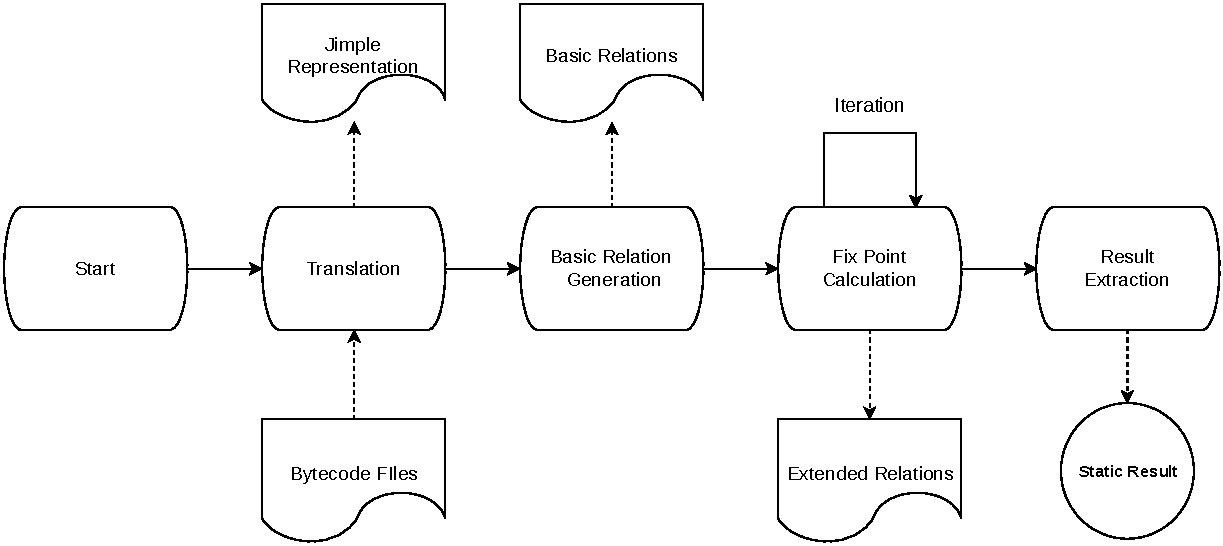
\includegraphics[width=16cm,height=6cm]{static-process.pdf}
\caption{Process of static analysis tool}
\label{fig:static-process}
\end{figure}

%% discuss shortly on array treatments, JDK/libraries, Reflection and JNI calls (moved from the next section)
In order to achieve an acceptable performance, we make conservative treatments on array accesses and library calls. We choose not to analyze method invocation from advanced Java language features such as reflection and JNI, and leave such calls as unresoled. Therefore, our methodology is unsound regarding these features, similar to most existing tools for Java program analysis, to the best of our knowledge (C.f.~an interesting discussion regarding soundiness~\cite{LivshitsSSLACGKMV15}). We will provide a detailed analysis regarding our conservative approach on the impact to the performance of our implemented TFA algorithm in Section~\ref{sec:evaluation}.



\subsection{Dynamic Profiling}\label{subsec:dynamic-profiler}

We apply dynamic analysis to collect the groundtruth of a program's run-time behaviour, such as the actual type a given variable has during an execution and the actual method being called at a particular program location. To build up a baseline for measuring the precision of TFA, we have implemented a dynamic profiling tool that records the actual types that a variable may have at run-time, in particular when the variable is a receiver at a call site. Based on the Soot framework, we instrument the jimple statements of the target benchmark programs that are subsequently tested in our experiment. After the instrumentation phase, run-time types are collected during the benchmark execution and are dumped to the output. We consider the collected variable-type relation as the groundtruth and compare it with the results generated by our static TFA algorithm, with details presented in section~\ref{subsec:accuracy}. In order to achieve effective instrumentation, we consider the following four possible ways on how to instrument a Java program.

%There are four manners to instrument the source code to record the run-time type of a method receiver.
%\begin{itemize}
%\item
\textbf{Insert First.}
%In this manner,
The type-recording statements are inserted as the first statement of each method block so that the type of \texttt{this} reference in that method will be recorded. %The reason we only have to record ``this'' reference is
Note that a receiver is always passed into \texttt{this} reference in a callee method, unless the method is static. %except for static methods.

\textbf{Insert Before.}
%Statements will be inserted before invocations and the type of receiver will be recorded in this manner. It is more straightforward than the method we discuss about recording ``this'' reference.
New statements are inserted  before each call site to collect the receiver type. This is more straightforward than \emph{Insert First}, as we do not need to find the types of \texttt{this} variables in callees.

\textbf{Insert Last.}
%This manner is similar with
Similar to \emph{Insert First}, except that statements are inserted before the last statement of a method block. We also record the type of \texttt{this} reference. % in this way.

\textbf{Insert After. \emph{(our scheme)}}
%Statments will be inserted right after invocations and the type of receiver will be recorded. It is similar with ``Insert Before'', except that statements are inserted at different position. We take this manner in our implementation and the reason will be discuss in section ~\ref{subsubsec:instrument}
In this way we insert statements right after each call site to record the type of the receiver, which is similar to \emph{Insert Before}. We choose to adopt this scheme and the reason is given as follows.
%\end{itemize}
%\subsubsection{Insert First}\label{subsubsec:insert-first}
%In this manner, the type-recorded statements will be insert before the first statement of a method block and the type of ``this'' reference in that method will be recorded. The reason we only have to record ``this'' reference is that a receiver is always passed into ``this'' reference in a method, except for static methods.
%\subsubsection{Insert Before}\label{subsubsec:insert-before}
%Statements will be inserted before invocations and the type of receiver will be recorded in this manner. It is more straightforward than the method we discuss about recording ``this'' reference.
%\subsubsection{Insert Last}\label{subsubsec:insert-last}
%This manner is similar with ``Insert First'', except that statements are inserted after the last statement of a method block. We also record ``this'' reference in this way.
%\subsubsection{Insert After}\label{subsubsec:insert-after}
%Statments will be inserted right after invocations and the type of receiver will be recorded. It is similar with ``Insert Before'', except that statements are inserted at different position. We take this manner in our implementation and the reason will be discuss in section ~\ref{subsubsec:instrument}
%\subsubsection{Our Instrumentation Manner}\label{subsubsec:instrument}

%We take ``Insert After'' as our instrumentation manner. The reason is mainly
According to the Java specification, the first statement of each constructor should be either another constructor of its own or its super class. Therefore, we would get a \emph{JVM voilation} error if we instrument a statement before the first statement in a constructor. We illustrate this problem in an example given in Listing~\ref{lst:spec-constructor}. Due to this restriction, both \emph{Insert First} and \emph{Insert Before} schemes cannot be applied. For the remaining to schemes, we choose \emph{Insert After} over \emph{Insert Last} for the reason that a last statement could be appeared in many different kinds like a return statement, an exception throwing statement, or even an application terminating invocation. It will take more time to tackle this problem if we use the  \emph{Insert Last} scheme to implement our profiler. More details are displayed in an example in Listing~\ref{lst:last-statement}. We can easily insert at line 4 and line 8, for an exception throwing statement and a return statement, respectively. However, it requires significant time to recognize line 7 as a last statement of method $m1$ since it will terminate the whole application. As a result, we use \emph{Insert After} as our implementation manner so that a type can be more easier and straightforwardly collected and bundled with its receiver. %due to the reason. %that it's more straightforward.
As an example, the code before and after instrumentation are shown in Listing~\ref{lst:before-instru} and Listing~\ref{lst:after-instru}, respectively. For Listing~\ref{lst:after-instru}, at line $5$, the funtion $RecordUtils.id()$ takes an invocation expression ($invokeExprssion$) and a method receiver ($b$) as parameters and return an unique representation string for this invocation. In this example, the collected unique representation is \emph{A:m1:b:B:m2:4}, which stands for $b$ calls method $m2$ of class $B$, at line $4$ within method $m1$ of class $A$. It also shows that $b$ is of type $B$ at this program location.

\begin{minipage}{\linewidth}
\vspace{10pt}
\begin{lstlisting}[caption={Java specification on constructor},label={lst:spec-constructor}]
class A {
  public A() {
    //insert statements here will violate JVM specification
    super();	//invoke super class constructor
  }
  public A(int i) {
    //insert statements here will violate JVM specification
    this();    //inovke another constructor of its own
  }
}
\end{lstlisting}
\end{minipage}

\begin{minipage}{\linewidth}
\vspace{10pt}
\begin{lstlisting}[caption={Example code of \emph{Insert Last}},label={lst:last-statement}]
class A {
  public Obejct m1(int i) {
    if(i>0) {
      // insert here, right before an exception throwing statement
      throw new Exception(``i>0'');  
    }
    exit(); // this invocation terminates application
    // insert here, right before a return statement
    return null;  // insert before this statement
  }

  public void exit() {
    System.exit(0);  // this invocation terminates application
  }
}
\end{lstlisting}
\end{minipage}

\begin{minipage}{\linewidth}
\vspace{10pt}
\begin{lstlisting}[caption={Example code before our instrumentation},label={lst:before-instru}]
class A {
  public void m1() {
    B b = new B();
    b.m2();    //invocation here
  }
}
\end{lstlisting}
\end{minipage}

\begin{minipage}{\linewidth}
\vspace{10pt}
\begin{lstlisting}[caption={Example code after our instrumentation},label={lst:after-instru}]
class A {
  public void m1() {
    B b = new B();
    b.m2();    //invocation here
    String record = RecordUtils.id(invokeExpression, b);
    RecordUtils.record(record);
  }
}
\end{lstlisting}
\end{minipage}

Test cases we use to trigger the program are officially provided by those benchmarks. Since static analysis would calculate all possible path of a program, those uncovered code of dynamic execution would possibly raise up imprecision for static analysis. We use method coverage as an index of code coverage and present it in Figure~\ref{fig:coverage}. These test cases can cover most of the defined methods on the majority of benchmarks. However, for some benchmarks, the test cases missed plenty of defined methods. Focus on the first benchmark $check$, there are $18$ methods not being executed at runtime. We have investigated why these methods are missed and realized there are tow reason leading to this problem. We pick some real code to explain, as shown in Listing~\ref{lst:uncovered-method}. As we known, SPECjvm2008~\cite{specjvm} provides multithreading mode to run the benchmarks, in order to test the computer performance. It defines some specify methods which will be executed under this mode, such as the method $testType()$ at line 2. Since we run the benchmarks on single threading mode, these methods would not be executed at runtime. For another reason that raise up the number of uncovered methods, some classes are designed as a pattern for different children classes. These pattern classes generally implements numerous inheriting methods from interface, tricklly doing nothing on their implementation. In this way, children classes could simply extend these pattern classes and override a few of methods. Note that interface`s method has to be all implemented on a non-abstract class. Therefore, if the children classes directly extend the original interface, they have to implement all the inheriting methods, even those they do not need at all. In Listing~\ref{lst:uncovered-method}, class $BaseFileObject$ extends interface $JavaFileObject$ and implements $13$ methods by simply throwing an exception. These methods would not be executed. $CachedFileObject$ and $OutputFileObject$ are two children classes extending $BaseFileObject$, they each only override one method of parent (\ie $getKind()$ at line 23 and $openOutputStream()$ at line 28). 

\begin{figure}\centering
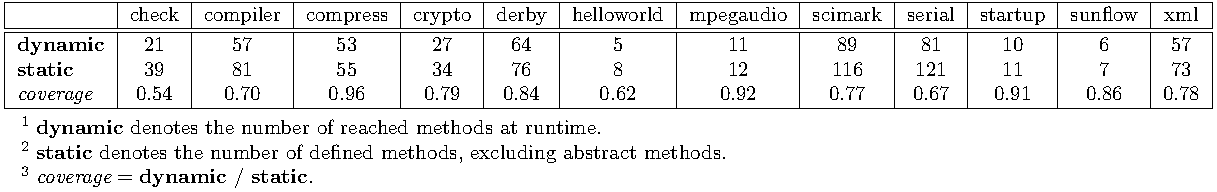
\includegraphics[scale=0.83]{coverage.pdf}
\caption{Method coverage for test cases}
\label{fig:coverage}
\end{figure}

\begin{minipage}{\linewidth}
\vspace{10pt}
\begin{lstlisting}[caption={Example code for uncovered methods },label={lst:uncovered-method}]
public class Main extends SpecJVMBenchmarkBase{
  public String testType() {
        return "multi";
  }
}

public class BaseFileObject implements JavaFileObject {
  public Kind getKind() {			
			throw new UnsupportedOperationException("getKind()");
		}
		
  public OutputStream openOutputStream() throws IOException {
			throw new UnsupportedOperationException("openOutputStream()");
		}
  // still 11 methods below which is defined in interface "JavaFileObject",
  // thus this class have to implement them even they are never being executed.
  ...
  ...
}

public class CachedFileObject extends BaseFileObject {		
  Kind kind;	
  public Kind getKind() {
		return kind;
  }
}
public class OutputFileObject extends BaseFileObject {
  public OutputStream openOutputStream() throws IOException {
    ...
  }
}
\end{lstlisting}
\end{minipage}

\section{Evaluation}\label{sec:evaluation}
We evaluate our approach by measuring its performance on SPECjvm2008~\cite{specjvm}, which consists of $12$ benchmark programs in total. We conduct our experiment on a laptop equipped with an Intel i5-8250U CPU at 1.60 GHz and 8 GB memory, running Ubuntu 16.04LTS with OpenJDK 1.8.0.

We compare our approach against Class Hierarchy Analysis (CHA) , Variable Type Analysis (VTA) and context-insensitive points-to analysis (PTA). Among these compared approaches, we use the hierarchy structure provided in Soot framework to implement CHA. The VTA and the points-to analysis are available from the Soot framework, which are both implemented by Soot team. We discover that since the VTA implementation in Soot is only an optional subprocess used to generat callgraph for points-to analysis, only the generated call graph is accessible by developer, and the general application interface of VTA is invisible to normal Soot users. Due to this restriction, we are unable to apply VTA as an independent process to measure its performance on the SPECjvm2008 benchmark programs. Nevertheless, we manage to compare precision and recall of our results with the call graph that is generated by the VTA subprocess, as shown in Figure~\ref{fig:recall} and Figure~\ref{fig:precision}.

The choice of comparing with the context-insensitive points-to analysis implementation in Soot is due to our approach also being context-insensitive. Therefore, the results from both approaches are comparable. In particular, the iterative algorithm for points-to analysis %to calculate a fixpoint due to the same reason.
provided by the Soot team adopts a more space-efficient \emph{bit vector} data structure to avoid \emph{Out-Of-Memory} error, 
as the points-to computation usually consumes more memory than TFA. For the implementation of TFA, we apply the usual data structure (\ie $HashSet$).
%
%A more space-efficient data structure for iteration set is adopted on points-to analysis, which is provided by Soot team. For the reason that points-to analysis will raise $OutOfMemory$ error and crash when we use the same data structure (\ie, $HashSet$) as in our implementation of TFA.

In the following tables listed in Figure~\ref{fig:TimeCost}, Figure~\ref{fig:recall} and Figure~\ref{fig:precision}, we use the keywords \textbf{CHA}, \textbf{VTA}, \textbf{PTA} and \textbf{TFA} to refer to the results from class hierarchy analysis, variable type analysis, points-to analysis and type flow analysis, respectively. During the evaluation the following two research questions are addressed. %%\fbox{TBD}
\begin{itemize}
\item \textbf{RQ1} How efficient is our type flow analysis based approach compared with the traditional class hierarchy analysis and points-to analysis?
\item \textbf{RQ2} How accurate is our algorithm comparing with the other approaches?
\end{itemize}
We try to provide answers to these two questions as discussed in section~\ref{subsec:efficiency} and section~\ref{subsec:accuracy}, respectively.

\subsection{Analysis on Performance}\label{subsec:efficiency}

We have executed all SPECjvm2008 benchmark programs $10$ times with the CHA, PTA and TFA algorithms. Then we calculate the average time consumption (in seconds) as displayed at column \textbf{T$_{CHA}$}(s), \textbf{T$_{PTA}$}(s) and \textbf{T$_{TFA}$}(s) of the Table in Figure~\ref{fig:TimeCost}. We also list the sizes of the generated relations (\ie, the type flow relation `$\tflow$', variable partial order `$\less$' and the field access relation `$\hflow$'), which provide an estimation of input size for the problems we are treating. The result confirms that our approach consumes more time than CHA, which is reasonable, as CHA does not apply any propagation on types, but only analyzes the class and interface hierarchy structure.\footnote{Note that we have implemented the current CHA algorithm by using the class hierarchy structure provided in the Soot framework. The default CHA implementation in Soot runs much slower, as shown in our earlier experiment result in~\cite{ZhuoZ19}.} TFA is in general more efficient than points-to analysis. In general, the runtime cost of TFA increases on benchmarks with larger size of generated relations as well as higher relational complexity, as most of the time in TFA is spent on calculating a fixpoint (\eg, on benchmark $check$ the number of generated relations reach to $34,406$, on which TFA spends the most amount of time($3.52s$) among all benchmarks). We conjecture that PTA is slower than TFA because it requires extra time for maintaining and updating a heap abstraction.

\begin{figure}
\centering
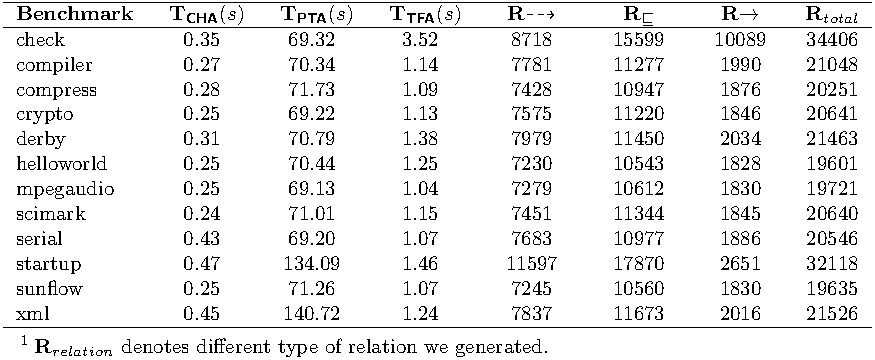
\includegraphics[scale=1]{timecost.pdf}
\caption{Runtime cost with different analysis}
\label{fig:TimeCost}
\end{figure}

\subsection{Analysis on Accuracy}\label{subsec:accuracy}

In this section we address the second question about accuracy in two perspectives: recall and precision. Firstly, the definitions are given in Equation~\ref{eq:recall} and Equation~\ref{eq:precision}, respectively.
\begin{equation}\label{eq:recall}
recall = \dfrac{TP}{TP+FN}
\end{equation}
\begin{equation}\label{eq:precision}
precision =  \dfrac{TP}{TP+FP}
\end{equation}
Here, $TP$ stands for \emph{true positive} which refers to the number of call edges identified by the analysis which also happens during program execution. $FN$ stands for \emph{false negative}, which is the number of call edges missed by the analysis. $FP$ (\emph{false positive}) refers to the number of call edges erroneously generated by the analysis. In general, a sound analysis should catch all existing runtime type information, \ie, the \emph{recall} should be $100\%$. On the other hand, \emph{precision} is defined as percentage of reported types that are correctly generated by the analysis. In general, given \emph{recall} fixed, a more precise algorithm should generate a smaller set of types for each calling variable. %%That is, $FP$ will be reduced.
We present recall and precision of the given approaches in Figure~\ref{fig:recall} and Figure~\ref{fig:precision}, respectively.


\begin{figure}\centering
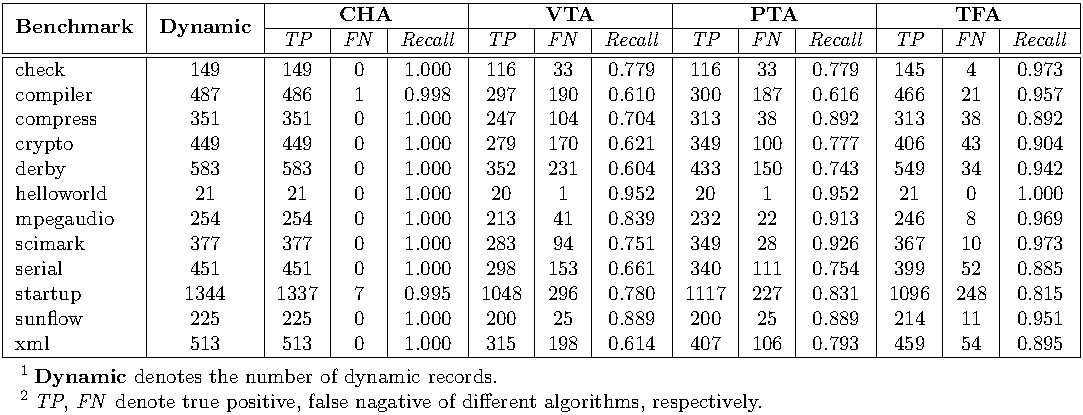
\includegraphics[scale=0.9]{recall-lib.pdf}
\caption{Recall on different analysis}
\label{fig:recall}
\end{figure}

\begin{figure}\centering
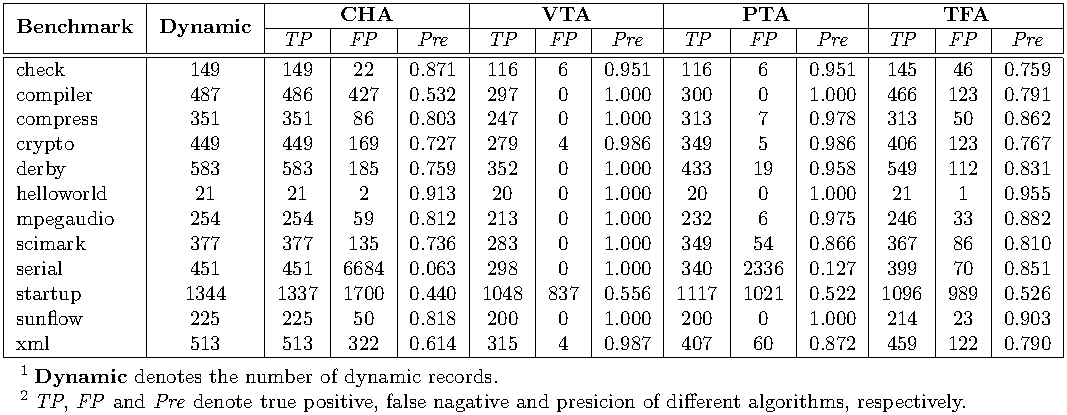
\includegraphics[scale=0.9]{precision-lib.pdf}
\caption{Precision of different analysis}
\label{fig:precision}
\end{figure}

%%discussion over recall

Regarding soundness, we use the call edges generated by the dynamic profiler (described in Section~\ref{subsec:dynamic-profiler}) as baseline, shown at the \textbf{Dynamic} columns of Figure~\ref{fig:recall} and Figure~\ref{fig:precision}. In general, CHA is able to achieve nearly $100\%$ recall, but VTA, TFA and PTA all fail to achieve $100\%$ recall except for the \texttt{helloworld} program. TFA is able to achieve above $90\%$ recall on average, higher than VTA and PTA ($20\%$ more recall on about half of the benchmark programs). Regarding precision, TFA archieves about $80\%$ on average, lower than VTA and PTA, but in general higher than CHA.

Given that TFA achieves a higher recall than VTA and PTA, we have identified a few possible reasons. Firstly, VTA and PTA implemented by the Soot team have applied an on-the-fly reachability analysis which rules out a portion of methods which are reported as unreachable. Therefore the unreachable methods would not be analyzed, and variables receiving their type from JDK would be assigned with possible types based on the preprocessing from Soot. For TFA, we have implemented a conservative approach on JDK library functions which always returns the predefined types of the API together with all their subtypes. We also implemented a conservative array analysis which may contribute to higher recall as well as lower precision. We also note that we have not implemented any special treatment regarding advanced Java language features including Java Reflection API and Java Native Interface calls, as well as more detailed analysis in the JDK library and side effects produced by callbacks from invisible codes (\eg from JDK library and reflective calls), which all contribute to the existence of $FN$ instances, so that TFA does not produce a sound result (\ie $100\%$ recall) on most benchmark programs.\footnote{As we mentioned earlier, most existing tools for Java program analysis are not sound, but soundy~\cite{LivshitsSSLACGKMV15}.}
For a more detailed explanation regarding the conservative treatment implemented in TFA, we refer to Section~\ref{subsec:analysis}.

We have also investigated why CHA also missed $8$ call edges on the benchmarks \texttt{compiler} and \texttt{startup}. The one missed on \texttt{compiler} is caused by the incomplete default hierarchy structure provided by the Soot framework. As an example, we put on a hierarchy structure of $javax.tools.JavaFileManager\$Location$ in JDK, as shown in Figure~\ref{fig:cha-hierarchy}. Note that variable $x$ is declared of type $javax.tools.JavaFileManager\$Location$ in benchmark \texttt{compiler}. However, the hierarchy structure provided by the Soot framework does not properly include $javax.tools.DocumentationTool\$Location$ or $javax.tools.StandardLocation$ as subclassses of $javax.tools.JavaFileManager\$Location$. Hence, these $2$ types are missed by CHA for variable $x$. The other $7$ missed types in CHA are due to that the Soot framework mistakenly changes the name of a few temporary variables (\eg, variable $\$68$ is changed to $\$58$), which can be detected by inspecting the jimple representation of the benchmark \texttt{startup}. % and find out those mistaken variable do not appear in it.


%Note that CHA also misses $8$ records on $compiler$ and $startup$ in total. $1$ missed records on $compiler$ and is caused by the incomplete hierarchy structure which is defaultly provided in Soot framework. \eg, we put on a hierarchy structure of $javax.tools.JavaFileManager\$Location$ in JDK, as shown in Fig.~\ref{fig:cha-hierarchy}. On benchmark $compiler$, variable $x$ is declared as ``$javax.tools.JavaFileManager\$Location$''. The hierarchy structure provided by Soot framework do not include ``$javax.tools.DocumentationTool\$Location$ and ``$javax.tools.StandardLocation$''as subclassses of ``$javax.tools.JavaFileManager\$Location$''. Hence, these $2$ types will be missed for variable $x$. The rest $7$ missed records in CHA are produced by Soot framework mistakenly changing the name of variable (\eg, variable $\$68$ is changed to $\$58$). We confirm the reason by reading the Jimple representation and find out those mistaken variable do not appear in it.

\begin{figure}
\centering
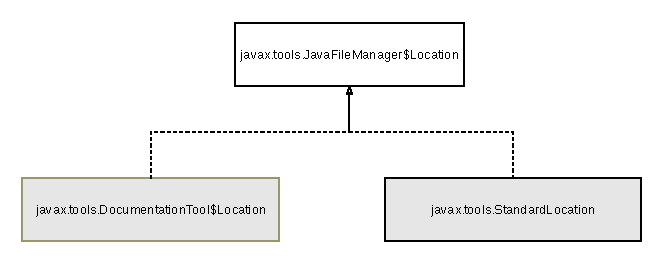
\includegraphics[scale=1]{cha-hierarchy.pdf}
\caption{A simple hierarchy in JDK}
\label{fig:cha-hierarchy}
\end{figure}

%%discussion over precision

For a comparison of the algorithms regarding precision, the experiment result has shown that in general TFA achieves higher precision than CHA (except for the benchmark \texttt{check} on which TFA's conservative treatment on JDK library has generated $40$ more FPs), since CHA simply includes all subclasses of a declared class to the result. At the same time, TFA produces lower precision than VTA and PTA due to its decisive trade-off between recall and precision. The imprecision is mainly due to the over approximation on library invocation and array (we defer a detailed discussion to section~\ref{subsec:analysis}). These conservative treatment has raised up recall but lowered precision at the same time. For example, on benchmark \texttt{compiler}, the recall of TFA achieves $0.957$, which is much higher than VTA($0.610$) and PTA($0.616$), as TFA catches more call edges than VTA($169$) and PTA($166$). As a result, TFA generates more $FP$ than VTA($123$) and PTA($123$), with a lower precision of $0.791$. Focusing on the benchmark \texttt{serial} and \texttt{startup} as shown in Figure~\ref{fig:precision}, we notice that PTA has generated lots of FPs, which lowers its precision to $0.127$ and $0.522$. This is caused by Soot's conservative treatment on Java $Exception$ and its preprocessing on some specific library calls. %%% wait: We discuss it in section~\ref{subsubsec:exception} and section~\ref{subsubsec:pta-preprocess}.



%We analyzed those missed records and find out the reason is due to some Java advance features, liked reflection call and JNI call, which we will describe in section~\ref{subsubsec:reflection-call} and section~\ref{subsubsec:jni-call}. In addition, callback mechanism will raise unsoundness under our treatment on reflection, JNI and library call. We will discuss it in section~\ref{subsubsec:callback}. The result shows that VTA and PTA produces lower recall than TFA in general. We study the reason for this gap from reading the source code of Soot and find out there are some different treatments that produce this result. The first one is the on-the-fly reachability analysis used on PTA implemented by Soot team. Method invoked by reflection, or invoked as a callback function inside reflection, JNI and library, will be denoted as unreachable under this analysis. As a consequence, some methods would not be analyzed by PTA. Note that even the unreachable method would not be analyzed, a variable receiving its type from JDK would be assigned to possible types based on the preprocessing from Soot. Such that the set of possible reaching types for these variables would not be empty. The second one is that our approach performs conservatively treatment on library. We will discuss it in section~\ref{subsubsec:library}. Moreover, we find out that VTA make inappropriate treatment on anonymous class which reduce its recall. We consider it as a bug produced by Soot team. More details will be illustrated in section~\ref{subsubsec:anonymous}. Note that CHA also misses $10$ records on $compiler, crypto, startup$ in total. The $3$ missed records on $compiler$ and $crypto$ are caused by the incomplete hierarchy structure which is defaultly provided in Soot framework. \eg, we put on a hierarchy structure of $java.security.KeyPairGenerator$ in JDK, as shown in Fig.~\ref{fig:cha-hierarchy}. On benchmark $crypto$, variable $x$ is declared as ``$java.security.KeyPairGenerator$''. The hierarchy structure provided by Soot framework do not include ``$DSAKeyPairGenerator$,``$DSAKeyPairGenerator\$Current$'' and ``$DSAKeyPairGenerator\$Legacy$'' as subclassses of ``$KeyPairGenerator$''. Hence, these $3$ types will be missed for variable $x$. The rest $7$ missed records in CHA are produced by Soot framework mistakenly changing the name of variable (\eg, variable $\$68$ is changed to $\$58$). We confirm the reason by reading the Jimple representation and find out those mistaken variable do not appear in it.


Due to the conservative approach on JDK library function, the TFA analysis achieves higher recall with the price of lower precision in comparison to VTA and PTA. Note that in theory context insensitive TFA is equivalent to context insensitive PTA and is more precise than VTA, as studied in Section~\ref{sec:type-flow-analysis}. In order to make the implementations more comparable, we modify the implementation of TFA by removing the library call approximation to JDK. As shown in Figure~\ref{fig:nolib-recall} and Figure\ref{fig:nolib-precision}, without the conservative treatment on JDK library, in general TFA has a comparable precision and recall to VTA and PTA on the given benchmark suite. To explain the reason that VTA and PTA marginally outperform TFA in a few benchmarks, we refer to the optimization processes implemented by the Soot team on array operations and certain reflective calls that are exploited by the VTA and PTA processes.

\begin{figure}\centering
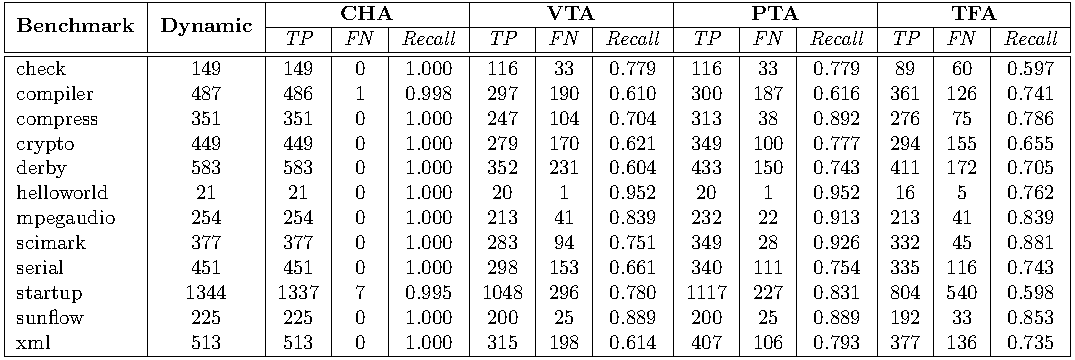
\includegraphics[scale=0.9]{recall-no-lib.pdf}
\caption{Recall without library approximation}
\label{fig:nolib-recall}
\end{figure}

\begin{figure}\centering
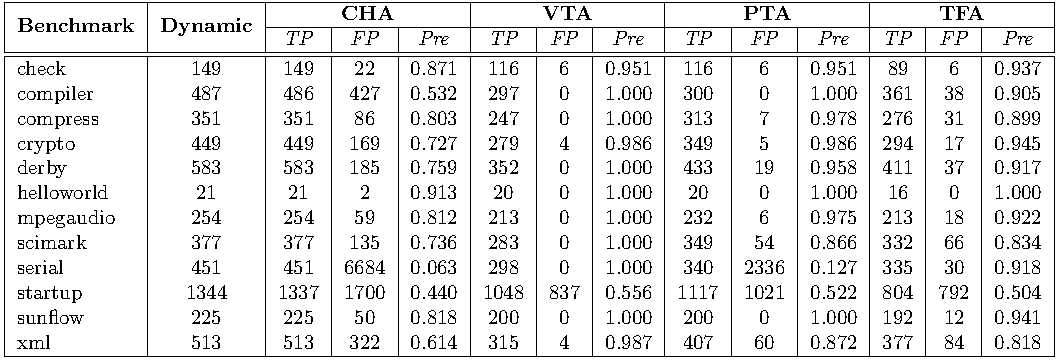
\includegraphics[scale=0.9]{precision-no-lib.pdf}
\caption{Precision without library approximation}
\label{fig:nolib-precision}
\end{figure}

\subsection{A Detailed Analysis on TFA's FP and FN}\label{subsec:analysis}

%\begin{figure}
%\centering
%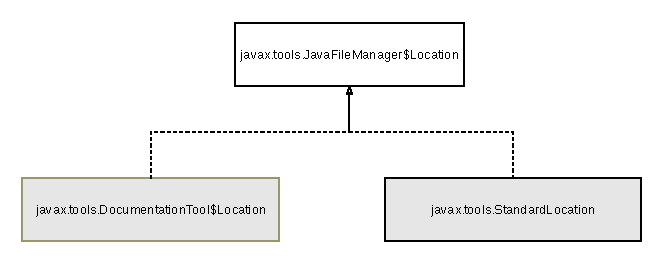
\includegraphics[scale=0.6]{cha-hierarchy.pdf}
%\caption{A simple hierarchy in JDK}
%\label{fig:cha-hierarchy}
%\end{figure}

%The result shows that in general our approach can achieve higher precision than CHA since CHA includes all the subclass of a declared class to the result. At the same time, it produce lower precision than VTA and PTA because of the trade-off between recall and precision. The imprecision is mainly due to our approximation on library invocation and array, which we will discuss in section~\ref{subsubsec:library} and section~\ref{subsubsec:array-approximation}. These conservative treatment would raise up our recall, but lower our precision in the meantime. \eg, on benchmark $compiler$, the recall of our method can achieve $0.955$, which is much higher than VTA($0.595$) and PTA($0.616$). For the reason that we catch more records than VTA($175$) and PTA($165$). As a result, we generated extra more records than VTA($89$) and PTA($96$), which reduces our precision to $0.829$.
%Focus on the benchmark $serial$ and $startup$ in Fig.~\ref{fig:precision}. We notice that PTA would generate lots of false positive, which lower its precision to $0.014$ and $0.386$. This is caused by Soot's conservative treatment on Java $Exception$ and preprocess on some specific library calls. We discuss it in section~\ref{subsubsec:exception} and section~\ref{subsubsec:pta-preprocess}.


%\begin{figure}\centering
%%\begin{table}[!htbp]\centering
%\begin{threeparttable}[b]
%\begin{tabular}{lcccccccccc}
%	\fullhline
%	\textbf{Benchmark} & \textbf{D} & \textbf{M$_{CHA}$} & \textbf{M$_{PTA}$} & \textbf{M$_{TFA}$} & \textbf{R$_{CHA}$} & \textbf{R$_{PTA}$} & \textbf{R$_{TFA}$} & \textbf{P$_{CHA}$} & \textbf{P$_{PTA}$} & \textbf{P$_{TFA}$} \hspace{2pt}\\
%	\fullhline
%check & 149 & 149 & 146 & 146 & 1.00 & 0.98 & 0.98 & 0.360 & 1.000 & 1.000\\
%compiler & 487 & 487 & 467 & 480 & 1.00 & 0.96 & 0.99 & 0.538 & 1.000 & 1.000\\
%compress & 351 & 351 & 339 & 347 & 1.00 & 0.97 & 0.99 & 0.793 & 1.000 & 1.000\\
%crypto & 449 & 449 & 402 & 413 & 1.00 & 0.90 & 0.92 & 0.732 & 1.000 & 1.000\\
%derby & 583 & 583 & 565 & 580 & 1.00 & 0.97 & 0.99 & 0.284 & 1.000 & 0.900\\
%helloworld & 21 & 21 & 21 & 21 & 1.00 & 1.00 & 1.00 & 0.167 & 1.000 & 1.000\\
%mpegaudio & 254 & 254 & 247 & 251 & 1.00 & 0.97 & 0.99 & 0.500 & 1.000 & 1.000\\
%scimark & 377 & 377 & 366 & 368 & 1.00 & 0.97 & 0.98 & 0.523 & 1.000 & 1.000\\
%serial & 451 & 451 & 399 & 407 & 1.00 & 0.88 & 0.90 & 0.000 & 1.000 & 1.000\\
%startup & 1344 & 1343 & 1289 & 1289 & 1.00 & 0.96 & 0.96 & 0.131 & 0.167 & 1.000\\
%sunflow & 225 & 225 & 215 & 219 & 1.00 & 0.96 & 0.97 & 0.440 & 1.000 & 1.000\\
%xml & 513 & 513 & 466 & 505 & 1.00 & 0.91 & 0.98 & 0.609 & 1.000 & 0.738\\
%	\fullhline
%\end{tabular}
%\caption{Accuracy with different analysis}
%\label{fig:accuracy}
%\begin{tablenotes}
%  \item[1] \textbf{D} denotes dynamic records.
%  \item[2] \textbf{M$_{algorithm}$}, \textbf{R$_{algorithm}$}, \textbf{P$_{algorithm}$} denote matching count, recall and precision of different algorithms, respectively.
%\end{tablenotes}
%\end{threeparttable}
%%\end{table}
%\end{figure}

In this section we briefly review the factors that hamper the performance of our type flow analysis.

%\subsubsection{Reflection Call}\label{subsubsec:reflection-call}
\paragraph{Reflective calls.} Reflection is an advanced feature in the Java programming language which provides the ability to inspect and manipulate a Java class at runtime. It brings in extra complexity to programs and its behaviour is hard to predict statically. In Listing~\ref{lst:reflection} we show a sample code using reflection in one of the benchmark programs to discuss how reflection works and what our treatment is. Note that this is an example we have simplified from the real code in order to concentrate on the main functionality of reflection. We discuss in three cases.
\begin{itemize}
\item Object Creation.
From line $6$ to line $10$, a new obejct of type $SPECJVMBenchmarkBase$ is created by method $newInstance()$ on variable $c$ at line $10$, where $c$ is an object of $Constructor$ type and it refers to a specific constructor of class $SPECJVMBenchmarkBase$. In the TFA analysis, we discard the type information of the new object in such a case because it is usually difficult to statically identify which constructor is invoked. For example, At line $6$, if statement $Class.forName()$ receives a string argument from the outside such as file input and user input, it is usually not easy to find out the real type of $benchmarkClass$. As a result, the run time type of $c$ and $benchmark$ cannot be identified.
\item Method Invocation.
After a new object is instantiated, we can get an object of $Method$ type, referring to a specific method of a class, and call this method by the method $invoke()$ (line $17$). This effect is similar to a normal invocation at line $12$. The invocation receiver is passed to the first argument of $invoke()$. In a case of static invocation, a \textbf{null} reference is passed to the first argument. We do not consider this way of reflective method invocation in TFA, for the same reason as we discuss about object creation.
\item Field Modification.
The way to change a field using reflection is similar to processing method invocation. The line $24-25$ illustrate changing value of field $f$ on object $benchmark$ to a new object. %We discard this effect as well because of the difficulty on analyzing which class holds the target field.
We do not handle this effect in TFA, either.
\end{itemize}

\begin{minipage}{\linewidth}
\vspace{10pt}
\begin{lstlisting}[caption={Example code of reflection},label={lst:reflection}]
public static void runSimple(Class benchmarkClass, String [] args) {
  ...
  ...
  Class[] cArgs = { BenchmarkResult.class, int.class };
  Object[] inArgs = { bmResult, Integer.valueOf(1)};
  Class benchmarkClass = Class.forName("spec.harness.SpecJVMBenchmarkBase");
  Constructor c = benchmarkClass.getConstructor(cArgs);

  // Object creation using reflection
  SpecJVMBenchmarkBase benchmark = (SpecJVMBenchmarkBase)c.newInstance(inArgs);
  // normal method invocation
  benchmark.harnessMain();

  // method invocation
  Method harnessMain = benchmarkClass.getMethod("harnessMain", new Class[]{});
  // just like line 11 but in reflection manner
  harnessMain.invoke(benchmark, new Object[]{});

  Method setup = benchmarkClass.getMethod( "setupBenchmark", new Class[]{});
  // static invocation
  setup.invoke(null, new Object[]{});

  // field modification
  Field f = benchmarkClass.getField("f");
  f.set(benchmark, new Object());
}
\end{lstlisting}
\end{minipage}

%\subsubsection{Java Native Interface Call}\label{subsubsec:jni-call}
\paragraph{JNI calls.} Java Native Interface (JNI) is a standard Java programming interface which provide ability for Java code to interoperate with application or library written in other programming languages, such as C, C++ or assembly. We show the usage of JNI in Listing~\ref{lst:jni}. Method $m()$ is defined as a native method and should not be implemented in Java. This program will load a native library named $lib$, in which the method $m()$ is implemented in a different program language. We do not consider JNI calls in our algorithm since the code is not written in Java. Analyzing that code and the communication between Java and other languages are out of our research scope. As a consequence, the effect of the invocation $a.m()$ at line $8$ is not analyzed by TFA.

\begin{minipage}{\linewidth}
\vspace{10pt}
\begin{lstlisting}[caption={Example code of JNI},label={lst:jni}]
public class A {
  public native void m();
  static {
    System.loadLibrary("lib");
  }
  public static void main(String[] args) {
    A a = new A();
    a.m(); <---
  }
}
\end{lstlisting}
\end{minipage}

%\subsubsection{Library}\label{subsubsec:library}

\paragraph{Library call.} Library calls included in an application (\eg, JDK libraries, third-party libraries) are usually in pre-compiled bit code format, and their source code is often large and not made explicitly available. Listing~\ref{lst:jdk} shows a common case of JDK invocation. We do not analyze the detailed logic inside library code which are written at line $10-11$. Instead, we perform an over approximation on library invocation, based on the method definition which appears at line $9$. We assume that library invocation will return the definition type and any subtype of this definition type as the result type. For Listing~\ref{lst:jdk}, $sb2$ will receive $\{StringBuilder,\ any\_subtype\_of\_StringBuilder\}$ as the set of reaching types under this strategy.

\begin{minipage}{\linewidth}
\vspace{10pt}
\begin{lstlisting}[caption={Example of JDK library call},label={lst:jdk}]
import java.lang.StringBuilder;

public void m() {
  StringBuilder sb = new StringBuilder();
  StringBuilder sb2 = sb.append("abc"); <---
}

//  @Override
//  public StringBuilder append(String str) {
//    ...
//    ...
//  }
\end{lstlisting}
\end{minipage}

%\subsubsection{Array Approximation}\label{subsubsec:array-approximation}
\paragraph{Array approximation.} We perform a conservative treatment on array accesses in the way that all type information that flows to one member of an array flows to all members of that array. Codes in Listing~\ref{lst:array} are used to explain how this approximation works. In this example, type information of $A$ and $B$ flow to the first member and the second member of array $arr$, respectively. We treat in the way that both $A$ and $B$ flow to the array $arr$, so that loadding an element of $arr$ receives both types (\ie $b$ receives $\{A, B\}$ as the set of reaching types, which is the same set of types that array $arr$ can access).

\begin{minipage}{\linewidth}
\vspace{10pt}
\begin{lstlisting}[caption={Example of array access},label={lst:array}]
public void m() {
	Object[] arr = new Object[2]{};
	arr[1] = new A();
	arr[2] = new B();
	Object b = arr[1];  <---
}
\end{lstlisting}
\end{minipage}

%\subsubsection{Callback}\label{subsubsec:callback}
\paragraph{Callbacks.} A callback function is known as a ``call-after'' function, which is widely used in object-oriented styled programming. By passing an argument to a method, the receiver may be used inside the callee to trigger a callback invocation. In functional language a callback funtion can be passed as argument directly. Listing~\ref{lst:callback}
illustrates the callback mechanism, where function $callback()$ of class $B$ is invoked after the invocation of $trigger()$ of class $A$. Since we do not analyze the effect of reflection calls, JNI calls and library calls, we are unable to catch the type flow information inside $a.trigger(b)$ if it happens to be one of these calls (\eg, $trigger()$ is a method of a library class). Note that we only conservatively approximate on the return type of a library invocation. %, but not analyze the detail logic inside a library method.

\begin{minipage}{\linewidth}
\vspace{10pt}
\begin{lstlisting}[caption={Callback mechanism},label={lst:callback}]
class A {
	public void trigger(B b) {
		b.callback();  // here the callback function actually executes
	}
}

class B {
	public void callback() {...}
	public void static main() {
		A a = new A();
		B b = new B();
		a.trigger(b);
 	}
}
\end{lstlisting}
\end{minipage}


%\subsubsection{Java Exception}
%\label{subsubsec:exception}
\paragraph{Exception handling.} PTA implemented by Soot conservatively add all the subclass of $Throwable$ to the possible types of variable $t$ if method $m()$ is reachable. Relevant code is shown in Listing~\ref{lst:exception}. Since $Throwable$ is the superclass of all errors and exceptions in Java. These result set could be pretty large. In general it would reach to more than $200$. That means if we only have a single dynamic record for this invocation statement, the precision will be reduced significantly.

\begin{minipage}{\linewidth}
\vspace{10pt}
\begin{lstlisting}[caption={Java Exception},label={lst:exception}]
class A {
	void m() {
		try {
			...
		} catch (Throwable t) {
			t.printStackTrace();
		}
	}
}
\end{lstlisting}
\end{minipage}

\newcommand\commentout[1]{}

\commentout{%%%BEGIN
\subsubsection{Preprocess of PTA}
\label{subsubsec:pta-preprocess}
\paragraph{The preprocessor by Soot.} Soot team performs a preprocess on some specific library calls, which aims to provide a sounder implementation of PTA. We pick up some code on the benchmark \texttt{serial} as shown in Listing~\ref{lst:pta-preprocess}, to describe why the precision of PTA is low on this benchmark. At line $5$, the reflective library call ``$method.invoke()$'', which is preprocessed by Soot framework. We put on the definition of this method in commented lines. The result of this preprocess is that $obj$ will receive its possible types as all the classes this method can return. We check out the number is generally reached to more than $1000$. \eg, on benchamrk $serial$, PTA generated more than $2000$ false positive cases and lower its precision to just $0.127$.

\begin{minipage}{\linewidth}
\vspace{10pt}
\begin{lstlisting}[caption={Preprocess of PTA},label={lst:pta-preprocess}]
class A {
	void m() {
		...
		Method method = getMethod();
		Object obj = method.invoke(null, new Object[]{});
		obj.getClass();
	}
}

//public Object invoke(Object obj, Object... args)
//        throws IllegalAccessException,IllegalArgumentException,
//				InvocationTargetException
//    {
//        ...
//    }
\end{lstlisting}
\end{minipage}

}%%%END

\section{Related Work}\label{sec:related-work}
There are not many works focusing on general purpose call graph construction algorithms, and we give a brief review of these works first.
%
As stated in the introduction, Class Hierarchy Analysis (CHA)~\cite{Dean1995,Fernandez1995}, Rapid Type Analysis (RTA)~\cite{Bacon1996} and Variable Type Analysis (VTA)~\cite{Sundaresan2000} are efficient algorithms that conservatively resolves call sites without any help from points-to analysis. Grove et al.~\cite{Grove1997} introduced an approach to model context-sensitive and context-insensitive call graph construction. They define call graph in terms of three algorithm-specific parameter partial orders, and provide a method called Monotonic Refinement, potentially adding to the class sets of local variables and adding new contours to call sites, load sites, and store sites.
%
Tip and Palsberg~\cite{Tip2000} Proposed four propagation-based call graph construction algorithms, CTA, MTA, FTA and XTA. CTA uses distinct sets for classes, MTA uses distinct sets for classes and fields, FTA uses distinct sets for classes and methods, and XTA uses distinct
sets for classes, fields, and methods. The constructed call graphs tend to contain slightly fewer method definitions when compared to RTA. It has been shown that associating a distinct set of types with each method in a class has a significantly greater impact on precision than using a distinct set for each field in a class. Reif et al.~\cite{Reif2016} study the construction of call graphs for Java libraries that abstract over all potential library usages, in a so-called \emph{open world} approach. They invented two concrete call graph algorithms for libraries based on adaptations of the CHA algorithm, to be used for software quality and security issues. In general they are interested in analyzing library without knowing client application, which is complementary to our work that has focus on client program while treating library calls as end nodes.

Call graphs may serve as a basis for points-to analysis, but often a points-to analysis implicitly computes a call graph on-the-fly, such as the context insensitive points-to algorithm implemented in Soot using SPARK~\cite{Lhotak2003}. Most context-sensitive points-to analysis algorithms (e.g.,~\cite{Milanova2005,Sridharan2006,Smaragdakis11,Tan16}) progress call edges together with value flow, to our knowledge. The main distinction of our approach from these points-to analysis is the usage of an abstract heap, as we are only interested in the actual reaching types of the receiver of a call. Nevertheless, unlike CHA and VTA, our methodology can be extended to context-sensitive~settings.

Regarding the treatment of flow analysis in our algorithm, downcast analysis has been studied in region inference which is a special memory management scheme for preventing dangling pointers or improving precision in garbage collection in object-oriented programming languages~\cite{Boyapati2003,Chin2004}.  These works are type-based analysis, while our methodology belongs to traditional static program analysis. Similar ideas regarding value flow can also be found in the graph-reachability based formulation (e.g.~\cite{Reps1997,Lu2013}) to which all distributed data flow analyses can be adopted.

Runtime profiling data can be recorded and used to compare with static analysis result. Furthermore, these runtime data can help static algorithms to increase precision and achieve adaptive ability. In general there are two ways to record runtime profiling data for Java programs, collecting from Java VM~\cite{Codrut2014}, or using program instrumentation technique to extract these data in runtime~\cite{Sundaresan2000}. Inspire by~\cite{Sundaresan2000}, and partialy due to Java VM can only internally provide the data we want, our dynamic type recorder is implemented using instumented technique.

Instrumentation for Java bytecode can be performed either statically or dynamically. Traditional instrumentation is executed statically at most time, which suffers from the limitation that dynamically generated code or downloaded code will be skiped from instrumentation. Walter et al.~\cite{Binder2007} implemented an framework called FERRARI which can perform instrumentation in both ways. However, our dynamic profiler is implemented using statically instrumentation. Hence, dynamically generated code can not be instrumented. We do not implemented dynamic instrumentation yet, but note that all the benchmarks code we tested are statically asscessible (\ie, none of codes are dynamically generated or downloaded).

\section{Conclusion and future work}\label{sec:conclusion}
In this paper we have proposed Type Flow Analysis (TFA), a new semantics that statically determines reaching types of variables and constructs a relatively precise call graph edges for Object-Oriented programming languages in an efficient way. We have proved that our method is as precise as subset-based points-to analysis, regarding type related information. The computation of TFA is purely relational, since it do not require a heap abstraction that is needed by a points-to analysis.

To evaluate our method in practice, we implement a static type analysis tool in Soot framework, which runs our algorithm. Moreover, a dynamic type profiler is used to extract run-time types of variables, which are then used to compare with static results. We implement it using instrumentation technique, abiding by specification of Java VM. We have compared our method with built-in CHA and points-to algorithms available in Soot regarding precision and recall. The result have shown that our method achieved promising result and it is confirmed that in general TFA is applicable in the type resultion problem for real world~applications.

There are still some works we can do to enhance our algorithm. On the theoretical aspect, we can develop our algorithm to context-sensitive, in a way similar to points-to analysis~\cite{Milanova2005,Smaragdakis11}. On the practical aspect, we can combine static result and dynamic result to make our algorithm more adaptive, inspire by the approach proposed in~\cite{Codrut2014}.

\paragraph{Acknowlegements} The authors thank Bernhard Scholz for his guidance in our experiment regarding JVM configurations. We also thank anonymous reviewers of ICFEM 2019 for their help suggestions.
\label{lastpage}

\bibliographystyle{alpha}
\bibliography{fac-reference}

\end{document}
